\documentclass[11pt,letterpaper]{article}

% =============================================================================
% PACKAGES
% =============================================================================
\usepackage[margin=1in]{geometry}
\usepackage{enumitem}
\usepackage{setspace}
\usepackage{graphicx}
\usepackage{xcolor}
\usepackage{tikz}
\usetikzlibrary{shapes.geometric, arrows.meta, positioning, fit, backgrounds, calc, decorations.pathreplacing, trees, matrix}
\usepackage{tcolorbox}
\usepackage{booktabs}
\usepackage{amsmath,amssymb}
\usepackage{longtable}
\usepackage{array}
\usepackage{tabularx}
\usepackage{multirow}
\usepackage{fancyhdr}
\usepackage{titlesec}
\usepackage[colorlinks=true,linkcolor=blue!60!black,urlcolor=blue!60!black,citecolor=blue!60!black]{hyperref}
\usepackage{bookmark}
\usepackage{parskip}
\usepackage{float}
\usepackage{caption}
\usepackage{subcaption}
\usepackage{listings}
\usepackage{microtype}
\usepackage{textcomp}
\usepackage{forest}

% =============================================================================
% CONFIGURATION
% =============================================================================
\setstretch{1.15}

% Define colors
\definecolor{primary}{RGB}{25, 84, 123}
\definecolor{secondary}{RGB}{60, 120, 160}
\definecolor{accent}{RGB}{200, 80, 60}
\definecolor{success}{RGB}{40, 140, 80}
\definecolor{lightgray}{RGB}{245, 245, 245}
\definecolor{darkgray}{RGB}{80, 80, 80}
\definecolor{modulecolor}{RGB}{230, 245, 255}
\definecolor{packagecolor}{RGB}{255, 245, 220}
\definecolor{interfacecolor}{RGB}{220, 255, 230}
\definecolor{layercolor1}{RGB}{255, 230, 230}
\definecolor{layercolor2}{RGB}{230, 255, 230}
\definecolor{layercolor3}{RGB}{230, 230, 255}
\definecolor{layercolor4}{RGB}{255, 255, 220}

% Section formatting
\titleformat{\section}{\Large\bfseries\color{primary}}{\thesection}{1em}{}[\titlerule]
\titleformat{\subsection}{\large\bfseries\color{secondary}}{\thesubsection}{1em}{}
\titleformat{\subsubsection}{\normalsize\bfseries\color{darkgray}}{\thesubsubsection}{1em}{}

% Header/Footer
\pagestyle{fancy}
\fancyhf{}
\fancyhead[L]{\small\textcolor{darkgray}{Development Viewpoint Specification}}
\fancyhead[R]{\small\textcolor{darkgray}{Architecture Documentation}}
\fancyfoot[C]{\thepage}
\renewcommand{\headrulewidth}{0.4pt}

% Custom environments
\newtcolorbox{definitionbox}[1][]{
    colback=lightgray,
    colframe=primary,
    fonttitle=\bfseries,
    title=#1,
    boxrule=0.5pt,
    arc=2pt,
    left=8pt,
    right=8pt,
    top=6pt,
    bottom=6pt
}

\newtcolorbox{examplebox}[1][]{
    colback=white,
    colframe=secondary,
    fonttitle=\bfseries,
    title=#1,
    boxrule=0.5pt,
    arc=2pt,
    left=8pt,
    right=8pt,
    top=6pt,
    bottom=6pt
}

\newtcolorbox{warningbox}[1][]{
    colback=orange!5,
    colframe=accent,
    fonttitle=\bfseries,
    title=#1,
    boxrule=0.5pt,
    arc=2pt,
    left=8pt,
    right=8pt,
    top=6pt,
    bottom=6pt
}

\newtcolorbox{guidancebox}[1][]{
    colback=green!5,
    colframe=success,
    fonttitle=\bfseries,
    title=#1,
    boxrule=0.5pt,
    arc=2pt,
    left=8pt,
    right=8pt,
    top=6pt,
    bottom=6pt
}

\newtcolorbox{patternbox}[1][]{
    colback=blue!3,
    colframe=primary!70,
    fonttitle=\bfseries,
    title=#1,
    boxrule=0.5pt,
    arc=2pt,
    left=8pt,
    right=8pt,
    top=6pt,
    bottom=6pt
}

% Listings configuration
\lstset{
    basicstyle=\ttfamily\small,
    backgroundcolor=\color{lightgray},
    frame=single,
    framerule=0.5pt,
    rulecolor=\color{darkgray},
    breaklines=true,
    captionpos=b,
    tabsize=2,
    showstringspaces=false,
    numbers=left,
    numberstyle=\tiny\color{darkgray},
    numbersep=5pt,
    xleftmargin=15pt
}

\lstdefinelanguage{yaml}{
    keywords={true,false,null,y,n},
    sensitive=false,
    comment=[l]{\#},
    morecomment=[s]{/*}{*/},
    morestring=[b]',
    morestring=[b]"
}

% Table column types
\newcolumntype{L}[1]{>{\raggedright\arraybackslash}p{#1}}
\newcolumntype{C}[1]{>{\centering\arraybackslash}p{#1}}
\newcolumntype{R}[1]{>{\raggedleft\arraybackslash}p{#1}}

% =============================================================================
% DOCUMENT BEGIN
% =============================================================================
\begin{document}

% Avoid hyperref duplicate page anchors due to titlepage resetting page counter
\hypersetup{pageanchor=false}

% -----------------------------------------------------------------------------
% TITLE PAGE
% -----------------------------------------------------------------------------
\begin{titlepage}
    \centering
    \vspace*{1.5cm}
    
    {\Huge\bfseries\color{primary} Development Viewpoint\par}
    \vspace{0.5cm}
    {\Large\color{secondary} Architecture Viewpoint Specification\par}
    \vspace{0.3cm}
    {\large\color{darkgray} Module Structure \& Implementation Organization\par}
    
    \vspace{1.5cm}
    
    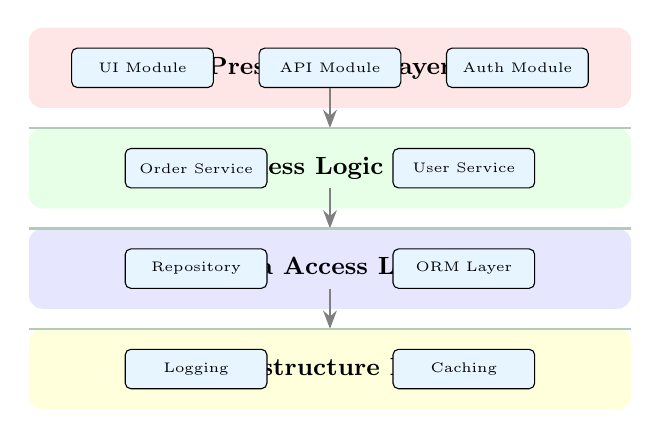
\begin{tikzpicture}[scale=0.85]
        % Layered architecture visualization
        \fill[layercolor1, rounded corners=5pt] (-4.5, 3) rectangle (4.5, 4.2);
        \node[font=\small\bfseries] at (0, 3.6) {Presentation Layer};
        
        \fill[layercolor2, rounded corners=5pt] (-4.5, 1.5) rectangle (4.5, 2.7);
        \node[font=\small\bfseries] at (0, 2.1) {Business Logic Layer};
        
        \fill[layercolor3, rounded corners=5pt] (-4.5, 0) rectangle (4.5, 1.2);
        \node[font=\small\bfseries] at (0, 0.6) {Data Access Layer};
        
        \fill[layercolor4, rounded corners=5pt] (-4.5, -1.5) rectangle (4.5, -0.3);
        \node[font=\small\bfseries] at (0, -0.9) {Infrastructure Layer};
        
        % Module boxes
        \node[draw, fill=modulecolor, rounded corners=2pt, minimum width=1.8cm, minimum height=0.5cm, font=\tiny] at (-2.8, 3.6) {UI Module};
        \node[draw, fill=modulecolor, rounded corners=2pt, minimum width=1.8cm, minimum height=0.5cm, font=\tiny] at (0, 3.6) {API Module};
        \node[draw, fill=modulecolor, rounded corners=2pt, minimum width=1.8cm, minimum height=0.5cm, font=\tiny] at (2.8, 3.6) {Auth Module};
        
        \node[draw, fill=modulecolor, rounded corners=2pt, minimum width=1.8cm, minimum height=0.5cm, font=\tiny] at (-2, 2.1) {Order Service};
        \node[draw, fill=modulecolor, rounded corners=2pt, minimum width=1.8cm, minimum height=0.5cm, font=\tiny] at (2, 2.1) {User Service};
        
        \node[draw, fill=modulecolor, rounded corners=2pt, minimum width=1.8cm, minimum height=0.5cm, font=\tiny] at (-2, 0.6) {Repository};
        \node[draw, fill=modulecolor, rounded corners=2pt, minimum width=1.8cm, minimum height=0.5cm, font=\tiny] at (2, 0.6) {ORM Layer};
        
        \node[draw, fill=modulecolor, rounded corners=2pt, minimum width=1.8cm, minimum height=0.5cm, font=\tiny] at (-2, -0.9) {Logging};
        \node[draw, fill=modulecolor, rounded corners=2pt, minimum width=1.8cm, minimum height=0.5cm, font=\tiny] at (2, -0.9) {Caching};
        
        % Dependency arrows
        \draw[-{Stealth}, thick, gray] (0, 3.3) -- (0, 2.7);
        \draw[-{Stealth}, thick, gray] (0, 1.8) -- (0, 1.2);
        \draw[-{Stealth}, thick, gray] (0, 0.3) -- (0, -0.3);
        
        % Interface indicators
        \draw[thick, interfacecolor!80!black] (-4.5, 2.7) -- (4.5, 2.7);
        \draw[thick, interfacecolor!80!black] (-4.5, 1.2) -- (4.5, 1.2);
        \draw[thick, interfacecolor!80!black] (-4.5, -0.3) -- (4.5, -0.3);
    \end{tikzpicture}
    
    \vspace{1.8cm}
    
    \begin{tabular}{ll}
        \textbf{Version:} & 2.0 \\
        \textbf{Status:} & Release \\
        \textbf{Classification:} & ISO/IEC/IEEE 42010 Compliant \\
        \textbf{Last Updated:} & \today \\
    \end{tabular}
    
    \vfill
    
    {\small Based on the Views and Beyond approach to software architecture documentation}
    
\end{titlepage}

% Re-enable page anchors for the rest of the document
\hypersetup{pageanchor=true}

% -----------------------------------------------------------------------------
% TABLE OF CONTENTS
% -----------------------------------------------------------------------------
\tableofcontents
\newpage

% =============================================================================
% SECTION: VIEWPOINT NAME
% =============================================================================
\section{Viewpoint Name}

\begin{definitionbox}[Viewpoint Identification]
\begin{tabular}{@{}L{3.5cm}L{10cm}@{}}
\textbf{Name:} & Development Viewpoint \\[0.5em]
\textbf{Synonyms:} & Implementation Viewpoint, Module Viewpoint, Code Structure Viewpoint, Logical Viewpoint, Static Structure View, Package Diagram View, Source Code Organization View \\[0.5em]
\textbf{Identifier:} & VP-DEV-001 \\[0.5em]
\textbf{Version:} & 2.0 \\
\end{tabular}
\end{definitionbox}

\subsection{Viewpoint Classification}

The Development Viewpoint belongs to the \textbf{Module Style} family within the Views and Beyond approach. It specifically addresses the static decomposition of software into implementation units, their organization, dependencies, and interfaces. This viewpoint is fundamental to understanding how the system is constructed and how development work can be organized.

\begin{table}[H]
\centering
\caption{Viewpoint Classification Taxonomy}
\begin{tabular}{@{}L{4cm}L{10cm}@{}}
\toprule
\textbf{Attribute} & \textbf{Value} \\
\midrule
Style Family & Module Styles \\
Primary Focus & Code Organization and Structure \\
Abstraction Level & Implementation/Code \\
Temporal Perspective & Development Time / Static Structure \\
Related Styles & Decomposition, Uses, Layered, Generalization \\
IEEE 42010 Category & Development Viewpoint \\
4+1 Equivalent & Development View \\
\bottomrule
\end{tabular}
\end{table}

\subsection{Viewpoint Scope}

The Development Viewpoint encompasses multiple related module styles, each emphasizing different structural relationships:

\begin{itemize}
    \item \textbf{Decomposition Style:} Shows how modules are decomposed into submodules, establishing a containment hierarchy that supports incremental development and information hiding.
    
    \item \textbf{Uses Style:} Documents the ``uses'' dependencies between modules, critical for determining build order, impact analysis, and identifying reusable components.
    
    \item \textbf{Layered Style:} Organizes modules into layers with controlled visibility and dependency rules, promoting separation of concerns and portability.
    
    \item \textbf{Generalization Style:} Captures inheritance and specialization relationships, supporting polymorphism and code reuse through object-oriented design.
    
    \item \textbf{Data Model Style:} Defines data entities, their attributes, and relationships, providing the structural foundation for persistent data.
\end{itemize}

% =============================================================================
% SECTION: OVERVIEW
% =============================================================================
\section{Overview}

The Development Viewpoint provides a comprehensive framework for documenting how a software system is organized into modules, packages, and other code units. This viewpoint is essential for managing complexity, enabling parallel development, supporting code reuse, and facilitating system evolution.

\subsection{Purpose and Scope}

The primary purpose of this viewpoint is to capture the static structure of the system's codebase---how implementation units are organized, how they relate to each other, and how they realize the system's functional and quality requirements. Unlike runtime views that show executing components, the Development Viewpoint focuses on the source code organization as it exists in the development environment.

\begin{definitionbox}[Viewpoint Definition]
The Development Viewpoint defines the static partitioning of a software system into modules, their interfaces, dependencies, and organizational structure. It provides the blueprint for code organization that supports development, testing, building, and maintaining the system throughout its lifecycle.
\end{definitionbox}

\subsection{Key Characteristics}

The Development Viewpoint exhibits several distinctive characteristics:

\textbf{Static Focus:} This viewpoint captures the system structure as it exists in source code repositories and build systems, independent of runtime behavior. It shows what code exists and how it is organized, not how it executes.

\textbf{Hierarchical Decomposition:} Modules are typically organized into hierarchies through decomposition and containment relationships. This hierarchy enables divide-and-conquer strategies for both understanding and developing the system.

\textbf{Dependency Management:} A central concern is understanding and managing dependencies between modules. Dependencies affect build order, change impact, testability, and the ability to develop modules independently.

\textbf{Interface Emphasis:} The viewpoint emphasizes module interfaces---what functionality each module exposes and what it requires from others. Well-defined interfaces enable loose coupling and independent development.

\textbf{Development Lifecycle Support:} The viewpoint directly supports development activities including coding, building, testing, version control, and team organization. Module boundaries often align with team boundaries.

\subsection{Relationship to Other Viewpoints}

The Development Viewpoint connects to other architectural viewpoints in important ways:

\begin{table}[H]
\centering
\caption{Relationships to Other Viewpoints}
\begin{tabular}{@{}L{3.5cm}L{10.5cm}@{}}
\toprule
\textbf{Viewpoint} & \textbf{Relationship} \\
\midrule
Component-and-Connector & Modules are packaged into runtime components. Module interfaces often map to component ports. \\
\addlinespace
Deployment & Modules are compiled into artifacts that get deployed. Build outputs become deployment units. \\
\addlinespace
Work Assignment & Module structure influences team organization. Module ownership maps to team responsibilities. \\
\addlinespace
Functional & Modules implement functional requirements. Module decomposition often follows functional decomposition. \\
\addlinespace
Quality Attribute & Module structure affects modifiability, testability, and reusability. Layer violations impact portability. \\
\addlinespace
Information/Data & Data model entities are implemented as modules. Data access patterns influence module dependencies. \\
\bottomrule
\end{tabular}
\end{table}

\subsection{Module Styles Overview}

\begin{figure}[H]
\centering
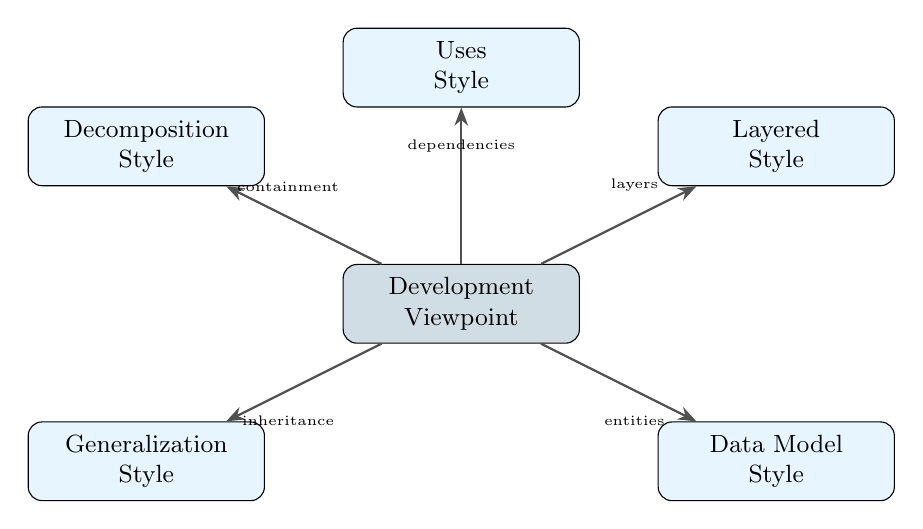
\begin{tikzpicture}[
    node distance=1.5cm and 2cm,
    style_node/.style={draw, fill=modulecolor, rounded corners=5pt, minimum width=3cm, minimum height=1cm, font=\small, align=center},
    arrow/.style={-{Stealth}, thick, darkgray}
]
    % Central node
    \node[style_node, fill=primary!20] (dev) at (0,0) {Development\\Viewpoint};
    
    % Style nodes
    \node[style_node] (decomp) at (-4, 2) {Decomposition\\Style};
    \node[style_node] (uses) at (0, 3) {Uses\\Style};
    \node[style_node] (layer) at (4, 2) {Layered\\Style};
    \node[style_node] (gen) at (-4, -2) {Generalization\\Style};
    \node[style_node] (data) at (4, -2) {Data Model\\Style};
    
    % Arrows
    \draw[arrow] (dev) -- (decomp);
    \draw[arrow] (dev) -- (uses);
    \draw[arrow] (dev) -- (layer);
    \draw[arrow] (dev) -- (gen);
    \draw[arrow] (dev) -- (data);
    
    % Labels
    \node[font=\tiny, anchor=south] at (-2.2, 1.3) {containment};
    \node[font=\tiny, anchor=south] at (0, 1.8) {dependencies};
    \node[font=\tiny, anchor=south] at (2.2, 1.3) {layers};
    \node[font=\tiny, anchor=north] at (-2.2, -1.3) {inheritance};
    \node[font=\tiny, anchor=north] at (2.2, -1.3) {entities};
\end{tikzpicture}
\caption{Development Viewpoint Style Family}
\end{figure}

% =============================================================================
% SECTION: CONCERNS
% =============================================================================
\section{Concerns}

This section enumerates the architectural concerns that the Development Viewpoint is designed to address. These concerns represent the fundamental questions that stakeholders have about the system's code organization and structure.

\subsection{Primary Concerns}

\begin{enumerate}[label=\textbf{C\arabic*:}, leftmargin=2.5em]
    \item \textbf{Code Organization and Structure}
    \begin{itemize}[nosep]
        \item How is the system decomposed into modules and packages?
        \item What is the hierarchical structure of the codebase?
        \item How are related functionalities grouped together?
        \item What naming conventions and organizational patterns are used?
        \item How does the structure support understanding and navigation?
    \end{itemize}
    
    \item \textbf{Module Dependencies and Coupling}
    \begin{itemize}[nosep]
        \item What dependencies exist between modules?
        \item Which modules are tightly vs. loosely coupled?
        \item Are there circular dependencies that need resolution?
        \item What is the impact of changing a specific module?
        \item How can dependencies be minimized or managed?
    \end{itemize}
    
    \item \textbf{Interface Design and Contracts}
    \begin{itemize}[nosep]
        \item What interfaces do modules expose?
        \item What contracts and invariants must implementations honor?
        \item How are interfaces versioned and evolved?
        \item What documentation exists for module APIs?
        \item How is interface stability ensured?
    \end{itemize}
    
    \item \textbf{Build and Compilation}
    \begin{itemize}[nosep]
        \item What is the build order for modules?
        \item How are build dependencies managed?
        \item What build tools and configurations are used?
        \item How are build artifacts organized and versioned?
        \item What are the compilation and linking requirements?
    \end{itemize}
    
    \item \textbf{Reusability and Sharing}
    \begin{itemize}[nosep]
        \item Which modules are designed for reuse?
        \item How are shared libraries and frameworks organized?
        \item What third-party dependencies are used?
        \item How is code duplication minimized?
        \item What modules can be extracted as independent libraries?
    \end{itemize}
    
    \item \textbf{Testability and Quality}
    \begin{itemize}[nosep]
        \item How does module structure support unit testing?
        \item Can modules be tested in isolation?
        \item What mocking and stubbing strategies are enabled?
        \item How is test code organized relative to production code?
        \item What quality metrics apply to module structure?
    \end{itemize}
    
    \item \textbf{Team Organization and Ownership}
    \begin{itemize}[nosep]
        \item Which teams own which modules?
        \item How does module structure enable parallel development?
        \item What coordination is required between teams?
        \item How are code review and approval boundaries defined?
        \item What expertise is required for each module?
    \end{itemize}
    
    \item \textbf{Evolution and Maintainability}
    \begin{itemize}[nosep]
        \item How easily can the system be modified?
        \item What is the expected rate of change for different modules?
        \item How are breaking changes managed?
        \item What refactoring opportunities exist?
        \item How is technical debt tracked and addressed?
    \end{itemize}
    
    \item \textbf{Standards and Conventions}
    \begin{itemize}[nosep]
        \item What coding standards apply?
        \item What architectural patterns are mandated?
        \item How is consistency enforced across modules?
        \item What documentation standards exist?
        \item How are exceptions to standards handled?
    \end{itemize}
\end{enumerate}

\subsection{Concern-Quality Attribute Mapping}

\begin{table}[H]
\centering
\caption{Concern to Quality Attribute Mapping}
\small
\begin{tabular}{@{}L{3.5cm}C{1.1cm}C{1.1cm}C{1.1cm}C{1.1cm}C{1.1cm}C{1.1cm}C{1.1cm}@{}}
\toprule
\textbf{Concern} & \rotatebox{60}{\textbf{Modifiability}} & \rotatebox{60}{\textbf{Testability}} & \rotatebox{60}{\textbf{Reusability}} & \rotatebox{60}{\textbf{Portability}} & \rotatebox{60}{\textbf{Buildability}} & \rotatebox{60}{\textbf{Understandability}} & \rotatebox{60}{\textbf{Performance}} \\
\midrule
Code Organization & $\bullet$ & $\circ$ & $\circ$ & $\circ$ & $\circ$ & $\bullet$ & -- \\
Dependencies & $\bullet$ & $\bullet$ & $\bullet$ & $\circ$ & $\bullet$ & $\circ$ & $\circ$ \\
Interfaces & $\bullet$ & $\bullet$ & $\bullet$ & $\bullet$ & $\circ$ & $\circ$ & -- \\
Build Process & $\circ$ & $\circ$ & $\circ$ & $\bullet$ & $\bullet$ & -- & -- \\
Reusability & $\circ$ & $\circ$ & $\bullet$ & $\bullet$ & $\circ$ & -- & -- \\
Testability & $\circ$ & $\bullet$ & $\circ$ & -- & $\circ$ & -- & -- \\
Team Organization & $\bullet$ & $\circ$ & $\circ$ & -- & $\circ$ & $\circ$ & -- \\
Evolution & $\bullet$ & $\circ$ & $\circ$ & $\circ$ & $\circ$ & $\circ$ & -- \\
\bottomrule
\multicolumn{8}{l}{\footnotesize $\bullet$ = Primary impact, $\circ$ = Secondary impact, -- = Minimal impact}
\end{tabular}
\end{table}

% =============================================================================
% SECTION: ANTI-CONCERNS
% =============================================================================
\section{Anti-Concerns}

Understanding what the Development Viewpoint is \emph{not} appropriate for helps stakeholders avoid misapplying this viewpoint.

\subsection{Out of Scope Topics}

\begin{enumerate}[label=\textbf{AC\arabic*:}, leftmargin=2.5em]
    \item \textbf{Runtime Behavior and Dynamics}
    \begin{itemize}[nosep]
        \item Process and thread execution models
        \item Message passing and event flows
        \item Runtime component interactions
        \item Dynamic object creation and lifecycle
        \item Concurrency and synchronization behavior
    \end{itemize}
    
    \item \textbf{Physical Infrastructure}
    \begin{itemize}[nosep]
        \item Hardware allocation and configuration
        \item Network topology and connectivity
        \item Server and container deployment
        \item Cloud infrastructure architecture
        \item Physical resource constraints
    \end{itemize}
    
    \item \textbf{User Interface Design}
    \begin{itemize}[nosep]
        \item Screen layouts and navigation flows
        \item Visual design and styling
        \item User experience patterns
        \item Accessibility requirements
        \item Responsive design breakpoints
    \end{itemize}
    
    \item \textbf{Business Process Workflows}
    \begin{itemize}[nosep]
        \item Business rule specifications
        \item Workflow state machines
        \item Process orchestration
        \item Business event sequences
        \item Approval and escalation chains
    \end{itemize}
    
    \item \textbf{Operational Procedures}
    \begin{itemize}[nosep]
        \item Deployment and release procedures
        \item Monitoring and alerting setup
        \item Incident response processes
        \item Backup and recovery procedures
        \item Performance tuning activities
    \end{itemize}
\end{enumerate}

\begin{warningbox}[Common Misapplications]
Avoid using the Development Viewpoint for:

\begin{itemize}[nosep]
    \item Documenting runtime component interactions (use C\&C Viewpoint)
    \item Specifying deployment topology (use Deployment Viewpoint)
    \item Defining user workflows (use Process/Functional Viewpoint)
    \item Planning release schedules (use Project Management tools)
    \item Detailing algorithm implementations (use detailed design documents)
\end{itemize}
\end{warningbox}

% =============================================================================
% SECTION: TYPICAL STAKEHOLDERS
% =============================================================================
\section{Typical Stakeholders}

The Development Viewpoint serves multiple stakeholder communities, each with distinct information needs and concerns about the system's code organization.

\subsection{Primary Stakeholders}

\begin{table}[H]
\centering
\caption{Primary Stakeholder Analysis}
\small
\begin{tabular}{@{}L{2.8cm}L{3.8cm}L{6.8cm}@{}}
\toprule
\textbf{Stakeholder} & \textbf{Role Description} & \textbf{Primary Interests} \\
\midrule
Software Architects & Design system structure and evolution & Module decomposition, dependency management, architectural patterns, quality attribute achievement \\
\addlinespace
Development Teams & Implement and maintain code & Module boundaries, interfaces, build processes, code navigation, testing strategies \\
\addlinespace
Tech Leads & Guide technical decisions & Coding standards, design patterns, technical debt, team coordination, code reviews \\
\addlinespace
Build Engineers & Manage build and CI systems & Build dependencies, compilation order, artifact management, build optimization \\
\addlinespace
Quality Engineers & Ensure code quality & Test organization, coverage analysis, static analysis, quality metrics \\
\addlinespace
Integration Teams & Integrate modules and systems & Interface contracts, integration points, dependency compatibility \\
\bottomrule
\end{tabular}
\end{table}

\subsection{Secondary Stakeholders}

\begin{table}[H]
\centering
\caption{Secondary Stakeholder Analysis}
\small
\begin{tabular}{@{}L{2.8cm}L{3.8cm}L{6.8cm}@{}}
\toprule
\textbf{Stakeholder} & \textbf{Role Description} & \textbf{Primary Interests} \\
\midrule
Project Managers & Plan and track delivery & Work breakdown, team allocation, dependency scheduling, progress tracking \\
\addlinespace
New Developers & Onboard to the codebase & System understanding, navigation, learning curve, documentation \\
\addlinespace
Security Analysts & Assess security posture & Attack surface, sensitive code locations, security module boundaries \\
\addlinespace
Performance Engineers & Optimize system performance & Hot paths, optimization targets, profiling boundaries \\
\addlinespace
Documentation Writers & Create technical docs & Module documentation, API references, architecture guides \\
\addlinespace
External Partners & Integrate with the system & Public APIs, SDK structure, extension points \\
\bottomrule
\end{tabular}
\end{table}

\subsection{Stakeholder Concern Matrix}

\begin{table}[H]
\centering
\caption{Stakeholder-Concern Responsibility Matrix}
\footnotesize
\begin{tabular}{@{}L{2.5cm}C{0.9cm}C{0.9cm}C{0.9cm}C{0.9cm}C{0.9cm}C{0.9cm}C{0.9cm}C{0.9cm}C{0.9cm}@{}}
\toprule
& \rotatebox{60}{\textbf{Organization}} & \rotatebox{60}{\textbf{Dependencies}} & \rotatebox{60}{\textbf{Interfaces}} & \rotatebox{60}{\textbf{Build}} & \rotatebox{60}{\textbf{Reusability}} & \rotatebox{60}{\textbf{Testability}} & \rotatebox{60}{\textbf{Teams}} & \rotatebox{60}{\textbf{Evolution}} & \rotatebox{60}{\textbf{Standards}} \\
\midrule
Architect & R & R & R & A & R & A & C & R & R \\
Dev Team & A & A & A & C & C & R & I & C & A \\
Tech Lead & A & A & A & C & A & A & R & A & A \\
Build Eng. & C & R & I & R & I & C & I & I & C \\
QA Engineer & I & C & C & C & I & R & I & C & C \\
Integration & C & A & R & C & C & C & I & C & I \\
\bottomrule
\multicolumn{10}{l}{\footnotesize R = Responsible, A = Accountable, C = Consulted, I = Informed}
\end{tabular}
\end{table}

% =============================================================================
% SECTION: MODEL TYPES
% =============================================================================
\section{Model Types}

The Development Viewpoint employs several complementary model types to capture different aspects of the code organization. Each model type serves specific documentation purposes.

\subsection{Model Type Catalog}

\begin{enumerate}[label=\textbf{MT\arabic*:}, leftmargin=2.5em]
    \item \textbf{Module Decomposition Diagram}
    \begin{itemize}[nosep]
        \item \textit{Purpose:} Show hierarchical decomposition of system into modules
        \item \textit{Primary Elements:} Modules, submodules, packages, containment
        \item \textit{Key Relationships:} Contains, is-part-of, decomposes-to
        \item \textit{Typical Notation:} UML Package Diagram, nested boxes
    \end{itemize}
    
    \item \textbf{Module Dependency Diagram}
    \begin{itemize}[nosep]
        \item \textit{Purpose:} Illustrate dependencies and uses relationships
        \item \textit{Primary Elements:} Modules, dependencies, interfaces
        \item \textit{Key Relationships:} Uses, depends-on, imports, requires
        \item \textit{Typical Notation:} UML Package Diagram with dependencies, directed graphs
    \end{itemize}
    
    \item \textbf{Layer Diagram}
    \begin{itemize}[nosep]
        \item \textit{Purpose:} Show layered organization with visibility rules
        \item \textit{Primary Elements:} Layers, modules within layers, bridges
        \item \textit{Key Relationships:} Allowed-to-use, is-above, bridges
        \item \textit{Typical Notation:} Stacked horizontal bands, layered boxes
    \end{itemize}
    
    \item \textbf{Class/Type Hierarchy Diagram}
    \begin{itemize}[nosep]
        \item \textit{Purpose:} Document inheritance and generalization structures
        \item \textit{Primary Elements:} Classes, interfaces, abstract types
        \item \textit{Key Relationships:} Extends, implements, generalizes
        \item \textit{Typical Notation:} UML Class Diagram (structure focus)
    \end{itemize}
    
    \item \textbf{Interface Specification}
    \begin{itemize}[nosep]
        \item \textit{Purpose:} Document module contracts and APIs
        \item \textit{Primary Elements:} Interfaces, operations, parameters, types
        \item \textit{Key Relationships:} Provides, requires, exposes
        \item \textit{Typical Notation:} API documentation, interface tables, OpenAPI
    \end{itemize}
    
    \item \textbf{Data Entity Model}
    \begin{itemize}[nosep]
        \item \textit{Purpose:} Define data structures and relationships
        \item \textit{Primary Elements:} Entities, attributes, relationships
        \item \textit{Key Relationships:} Has-a, references, contains
        \item \textit{Typical Notation:} ER diagrams, UML class diagrams (data focus)
    \end{itemize}
    
    \item \textbf{Build Dependency Graph}
    \begin{itemize}[nosep]
        \item \textit{Purpose:} Document build-time dependencies and order
        \item \textit{Primary Elements:} Build targets, artifacts, dependencies
        \item \textit{Key Relationships:} Depends-on, produces, consumes
        \item \textit{Typical Notation:} Directed acyclic graphs, build tool outputs
    \end{itemize}
    
    \item \textbf{Repository/Package Structure}
    \begin{itemize}[nosep]
        \item \textit{Purpose:} Show source code repository organization
        \item \textit{Primary Elements:} Repositories, directories, files, packages
        \item \textit{Key Relationships:} Contains, organized-in, co-located-with
        \item \textit{Typical Notation:} Tree diagrams, directory listings
    \end{itemize}
\end{enumerate}

\subsection{Model Type Relationships}

\begin{figure}[H]
\centering
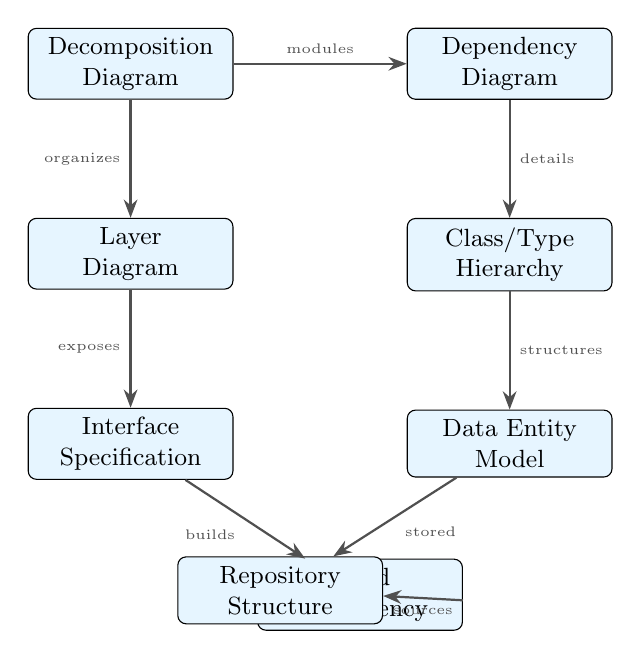
\begin{tikzpicture}[
    node distance=1.5cm and 2.2cm,
    model/.style={draw, fill=modulecolor, rounded corners=3pt, minimum width=2.6cm, minimum height=0.85cm, font=\small, align=center},
    arrow/.style={-{Stealth}, thick, darkgray}
]
    % Nodes
    \node[model] (decomp) {Decomposition\\Diagram};
    \node[model, right=of decomp] (depend) {Dependency\\Diagram};
    \node[model, below=of decomp] (layer) {Layer\\Diagram};
    \node[model, below=of depend] (class) {Class/Type\\Hierarchy};
    \node[model, below=of layer] (interface) {Interface\\Specification};
    \node[model, below=of class] (entity) {Data Entity\\Model};
    \node[model, below right=1cm and 0.3cm of interface] (build) {Build\\Dependency};
    \node[model, below left=1cm and 0.3cm of entity] (repo) {Repository\\Structure};
    
    % Arrows
    \draw[arrow] (decomp) -- (depend) node[midway, above, font=\tiny] {modules};
    \draw[arrow] (decomp) -- (layer) node[midway, left, font=\tiny] {organizes};
    \draw[arrow] (depend) -- (class) node[midway, right, font=\tiny] {details};
    \draw[arrow] (layer) -- (interface) node[midway, left, font=\tiny] {exposes};
    \draw[arrow] (class) -- (entity) node[midway, right, font=\tiny] {structures};
    \draw[arrow] (interface) -- (build) node[midway, below left, font=\tiny] {builds};
    \draw[arrow] (entity) -- (repo) node[midway, below right, font=\tiny] {stored};
    \draw[arrow] (build) -- (repo) node[midway, below, font=\tiny] {sources};
\end{tikzpicture}
\caption{Model Type Dependency Relationships}
\end{figure}

% =============================================================================
% SECTION: MODEL LANGUAGES
% =============================================================================
\section{Model Languages}

For each model type, specific languages, notations, and modeling techniques are prescribed. This section documents the vocabulary and grammar for constructing development views.

\subsection{UML Package Diagram Notation}

The Unified Modeling Language provides standardized notation for module structure through package diagrams.

\subsubsection{Primary Notation Elements}

\begin{table}[H]
\centering
\caption{UML Package Diagram Notation Elements}
\small
\begin{tabular}{@{}C{3cm}L{3.5cm}L{7cm}@{}}
\toprule
\textbf{Symbol} & \textbf{Element} & \textbf{Description} \\
\midrule
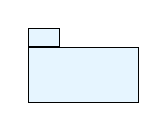
\begin{tikzpicture}[baseline=-0.5ex]
    \node[draw, fill=modulecolor, minimum width=1.4cm, minimum height=0.7cm] (p) {};
    \node[draw, fill=modulecolor, minimum width=0.4cm, minimum height=0.2cm, anchor=south west] at (p.north west) {};
\end{tikzpicture} & Package/Module & A namespace that groups related elements \\
\addlinespace
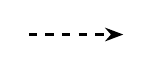
\begin{tikzpicture}[baseline=-0.5ex]
    \draw[thick, dashed, -{Stealth}] (0,0) -- (1.2,0);
\end{tikzpicture} & Dependency & One package depends on another \\
\addlinespace
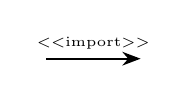
\begin{tikzpicture}[baseline=-0.5ex]
    \draw[thick, -{Stealth}] (0,0) -- (1.2,0);
    \node[font=\tiny] at (0.6, 0.2) {<<import>>};
\end{tikzpicture} & Import & Public import of package contents \\
\addlinespace
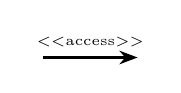
\begin{tikzpicture}[baseline=-0.5ex]
    \draw[thick, -{Stealth}] (0,0) -- (1.2,0);
    \node[font=\tiny] at (0.6, 0.2) {<<access>>};
\end{tikzpicture} & Access & Private access to package contents \\
\addlinespace
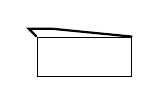
\begin{tikzpicture}[baseline=-0.5ex]
    \node[draw, fill=white, minimum width=1.2cm, minimum height=0.5cm] (n) {};
    \draw[thick] (n.north west) -- ++(-0.1, 0.1) -- ++(0.3, 0) -- (n.north east);
\end{tikzpicture} & Nested Package & Package contained within another \\
\bottomrule
\end{tabular}
\end{table}

\subsubsection{Package Stereotypes}

\begin{table}[H]
\centering
\caption{Common Package Stereotypes}
\small
\begin{tabular}{@{}L{3.5cm}L{10cm}@{}}
\toprule
\textbf{Stereotype} & \textbf{Description} \\
\midrule
\texttt{<<subsystem>>} & A large-scale package representing a major system division \\
\texttt{<<framework>>} & A reusable set of cooperating classes \\
\texttt{<<library>>} & A collection of utilities without application logic \\
\texttt{<<layer>>} & A horizontal slice of the architecture \\
\texttt{<<facade>>} & A package providing simplified interface to complex subsystem \\
\texttt{<<api>>} & A package containing public interface definitions \\
\texttt{<<implementation>>} & A package containing internal implementation details \\
\texttt{<<model>>} & A package containing domain model entities \\
\texttt{<<test>>} & A package containing test code \\
\bottomrule
\end{tabular}
\end{table}

\subsection{Layer Diagram Notation}

Layer diagrams use a specialized notation to show stratified organization:

\begin{figure}[H]
\centering
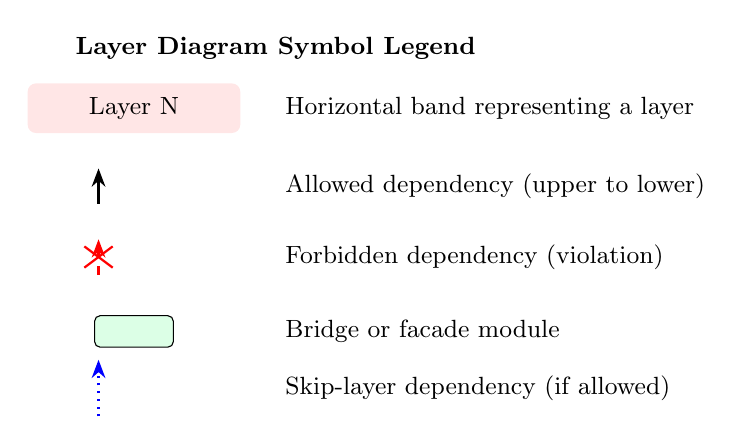
\begin{tikzpicture}[scale=0.9]
    % Legend
    \node[font=\small\bfseries] at (0, 5) {Layer Diagram Symbol Legend};
    
    % Layer representation
    \fill[layercolor1, rounded corners=3pt] (-3.5, 3.8) rectangle (-0.5, 4.5);
    \node[font=\small] at (-2, 4.15) {Layer N};
    \node[right, font=\small] at (0, 4.15) {Horizontal band representing a layer};
    
    % Allowed dependency
    \draw[thick, -{Stealth}] (-2.5, 2.8) -- (-2.5, 3.3);
    \node[right, font=\small] at (0, 3.05) {Allowed dependency (upper to lower)};
    
    % Forbidden dependency
    \draw[thick, -{Stealth}, red, dashed] (-2.5, 1.8) -- (-2.5, 2.3);
    \draw[red, thick] (-2.7, 1.9) -- (-2.3, 2.2);
    \draw[red, thick] (-2.7, 2.2) -- (-2.3, 1.9);
    \node[right, font=\small] at (0, 2.05) {Forbidden dependency (violation)};
    
    % Bridge/Facade
    \node[draw, fill=interfacecolor, rounded corners=2pt, minimum width=1cm, minimum height=0.4cm] at (-2, 1) {};
    \node[right, font=\small] at (0, 1) {Bridge or facade module};
    
    % Skip layer
    \draw[thick, -{Stealth}, blue, dotted] (-2.5, -0.2) -- (-2.5, 0.6);
    \node[right, font=\small] at (0, 0.2) {Skip-layer dependency (if allowed)};
\end{tikzpicture}
\caption{Layer Diagram Symbol Legend}
\end{figure}

\subsection{Dependency Notation Variants}

Different dependency types require different visual representations:

\begin{table}[H]
\centering
\caption{Dependency Type Notation}
\small
\begin{tabular}{@{}L{3cm}C{3cm}L{7.5cm}@{}}
\toprule
\textbf{Type} & \textbf{Notation} & \textbf{Meaning} \\
\midrule
Uses & 
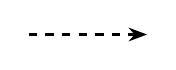
\begin{tikzpicture}[baseline=-0.5ex]
    \draw[thick, dashed, -{Stealth}] (0,0) -- (1.5,0);
\end{tikzpicture} & 
A requires B's correct functioning \\
\addlinespace
Implements & 
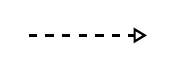
\begin{tikzpicture}[baseline=-0.5ex]
    \draw[thick, dashed, -{Triangle[open]}] (0,0) -- (1.5,0);
\end{tikzpicture} & 
A implements interface B \\
\addlinespace
Extends & 
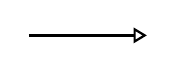
\begin{tikzpicture}[baseline=-0.5ex]
    \draw[thick, -{Triangle[open]}] (0,0) -- (1.5,0);
\end{tikzpicture} & 
A inherits from B \\
\addlinespace
Composes & 
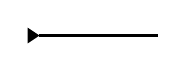
\begin{tikzpicture}[baseline=-0.5ex]
    \draw[thick] (0,0) -- (1.5,0);
    \fill (0,0) -- (-0.15,0.1) -- (-0.15,-0.1) -- cycle;
\end{tikzpicture} & 
A contains B (strong ownership) \\
\addlinespace
Aggregates & 
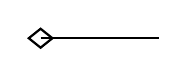
\begin{tikzpicture}[baseline=-0.5ex]
    \draw[thick] (0,0) -- (1.5,0);
    \draw[thick] (-0.15,0) -- (0,0.12) -- (0.15,0) -- (0,-0.12) -- cycle;
\end{tikzpicture} & 
A references B (weak ownership) \\
\addlinespace
Creates & 
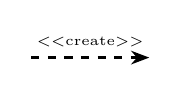
\begin{tikzpicture}[baseline=-0.5ex]
    \draw[thick, dashed, -{Stealth}] (0,0) -- (1.5,0);
    \node[font=\tiny] at (0.75, 0.2) {<<create>>};
\end{tikzpicture} & 
A instantiates B \\
\bottomrule
\end{tabular}
\end{table}

\subsection{Directory Structure Notation}

Source code organization is often documented using tree notation:

\begin{lstlisting}[caption={Directory Structure Example}, language={}]
project-root/
|-- src/
|   |-- main/
|   |   |-- java/
|   |   |   |-- com/
|   |   |       |-- example/
|   |   |           |-- domain/
|   |   |           |   |-- model/
|   |   |           |   |-- repository/
|   |   |           |-- service/
|   |   |           |-- controller/
|   |   |           |-- config/
|   |   |-- resources/
|   |-- test/
|       |-- java/
|       |-- resources/
|-- build.gradle
|-- settings.gradle
|-- README.md
\end{lstlisting}

\subsection{Interface Definition Languages}

Module interfaces can be specified using various formal languages:

\begin{table}[H]
\centering
\caption{Interface Definition Languages}
\small
\begin{tabular}{@{}L{2.8cm}L{3cm}L{7.7cm}@{}}
\toprule
\textbf{Language} & \textbf{Domain} & \textbf{Use Case} \\
\midrule
OpenAPI/Swagger & REST APIs & HTTP-based service interface definitions \\
GraphQL Schema & GraphQL APIs & Query and mutation type definitions \\
Protocol Buffers & gRPC Services & Binary serialization and RPC definitions \\
TypeScript Types & JavaScript/TS & Type definitions for JS modules \\
Java Interfaces & JVM Languages & Contract definitions for Java modules \\
C++ Headers & Native Code & Declaration files for C++ modules \\
IDL (CORBA) & Distributed Systems & Language-neutral interface definitions \\
WSDL & SOAP Services & XML-based web service descriptions \\
\bottomrule
\end{tabular}
\end{table}

\subsection{Tabular Module Specifications}

\subsubsection{Module Catalog Table}

\begin{table}[H]
\centering
\caption{Example Module Catalog Format}
\small
\begin{tabular}{@{}L{2.2cm}L{2.5cm}L{3cm}L{2.5cm}L{3cm}@{}}
\toprule
\textbf{Module ID} & \textbf{Name} & \textbf{Responsibility} & \textbf{Owner} & \textbf{Dependencies} \\
\midrule
MOD-001 & UserService & User management & Team Alpha & MOD-003, MOD-005 \\
MOD-002 & OrderService & Order processing & Team Beta & MOD-001, MOD-004 \\
MOD-003 & Repository & Data access & Team Alpha & MOD-006 \\
\bottomrule
\end{tabular}
\end{table}

\subsubsection{Interface Specification Table}

\begin{table}[H]
\centering
\caption{Example Interface Specification Format}
\small
\begin{tabular}{@{}L{2.5cm}L{2.5cm}L{3.5cm}L{2cm}L{2.5cm}@{}}
\toprule
\textbf{Operation} & \textbf{Parameters} & \textbf{Returns} & \textbf{Errors} & \textbf{Description} \\
\midrule
createUser & UserDTO & User & DuplicateError & Creates new user \\
getUser & userId: String & User | null & NotFoundError & Retrieves user \\
updateUser & userId, UserDTO & User & ValidationError & Updates user \\
deleteUser & userId: String & boolean & NotFoundError & Deletes user \\
\bottomrule
\end{tabular}
\end{table}

% =============================================================================
% SECTION: VIEWPOINT METAMODELS
% =============================================================================
\section{Viewpoint Metamodels}

This section defines the conceptual metamodel underlying the Development Viewpoint, establishing the vocabulary of element types, their properties, and valid relationships.

\subsection{Core Metamodel}

\begin{figure}[H]
\centering
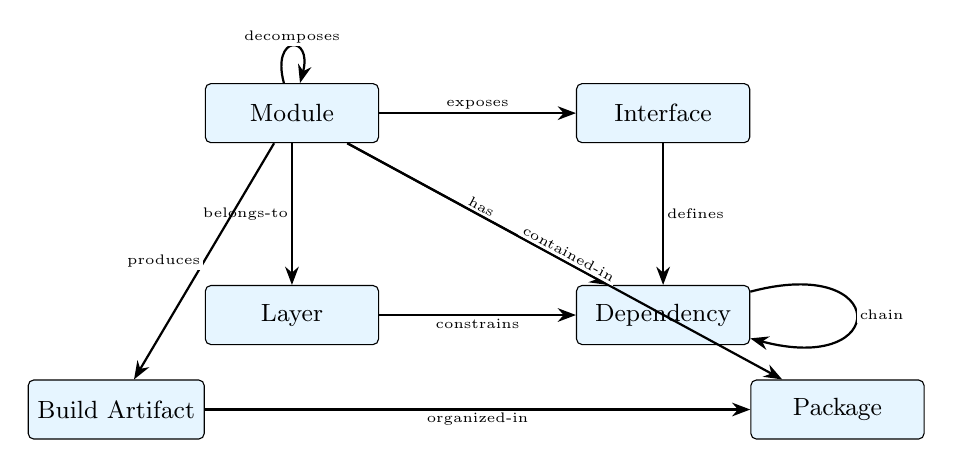
\begin{tikzpicture}[
    node distance=1.4cm and 2.2cm,
    entity/.style={draw, fill=modulecolor, rounded corners=2pt, minimum width=2.2cm, minimum height=0.75cm, font=\small},
    arrow/.style={-{Stealth}, thick},
    label/.style={font=\tiny, fill=white, inner sep=1pt}
]
    % Main entities
    \node[entity] (module) {Module};
    \node[entity, right=2.5cm of module] (interface) {Interface};
    \node[entity, below=1.8cm of module] (layer) {Layer};
    \node[entity, below=1.8cm of interface] (dependency) {Dependency};
    \node[entity, below left=3cm and 0cm of module] (artifact) {Build Artifact};
    \node[entity, below right=3cm and 0cm of interface] (package) {Package};
    
    % Relationships
    \draw[arrow] (module) -- (interface) node[label, midway, above] {exposes};
    \draw[arrow] (module) -- (layer) node[label, midway, left] {belongs-to};
    \draw[arrow] (module) -- (dependency) node[label, midway, above, sloped] {has};
    \draw[arrow] (interface) -- (dependency) node[label, midway, right] {defines};
    \draw[arrow] (module) -- (artifact) node[label, midway, left] {produces};
    \draw[arrow] (module) -- (package) node[label, midway, above, sloped] {contained-in};
    \draw[arrow] (layer) -- (dependency) node[label, midway, below] {constrains};
    \draw[arrow] (artifact) -- (package) node[label, midway, below] {organized-in};
    
    % Self-reference
    \draw[arrow] (module) to[loop above] node[label, above] {decomposes} (module);
    \draw[arrow] (dependency) to[loop right] node[label, right] {chain} (dependency);
\end{tikzpicture}
\caption{Development Viewpoint Core Metamodel}
\end{figure}

\subsection{Entity Definitions}

\begin{definitionbox}[Entity: Module]
\textbf{Definition:} A code unit that bundles related functionality and data, providing a well-defined interface and hiding implementation details.

\textbf{Attributes:}
\begin{itemize}[nosep]
    \item \texttt{moduleId}: Unique identifier for the module
    \item \texttt{name}: Human-readable name following naming conventions
    \item \texttt{type}: Classification (subsystem, component, library, utility)
    \item \texttt{responsibility}: Primary purpose and functionality provided
    \item \texttt{visibility}: Access level (public, internal, private)
    \item \texttt{version}: Current version identifier
    \item \texttt{owner}: Team or individual responsible for maintenance
    \item \texttt{status}: Development status (stable, experimental, deprecated)
    \item \texttt{qualityMetrics}: Code metrics (size, complexity, coverage)
\end{itemize}

\textbf{Constraints:}
\begin{itemize}[nosep]
    \item Each module must have a single, well-defined responsibility
    \item Module names must be unique within their containing package
    \item Public modules must have documented interfaces
    \item Cyclic dependencies between modules should be avoided
\end{itemize}
\end{definitionbox}

\begin{definitionbox}[Entity: Interface]
\textbf{Definition:} A contract that specifies the operations a module provides and the preconditions, postconditions, and invariants that govern their use.

\textbf{Attributes:}
\begin{itemize}[nosep]
    \item \texttt{interfaceId}: Unique identifier
    \item \texttt{name}: Interface name
    \item \texttt{version}: Interface version (semantic versioning)
    \item \texttt{operations}: List of operations/methods exposed
    \item \texttt{dataTypes}: Types used in the interface
    \item \texttt{preconditions}: Conditions that must hold before operations
    \item \texttt{postconditions}: Conditions guaranteed after operations
    \item \texttt{invariants}: Conditions that always hold
    \item \texttt{exceptions}: Error conditions that may be raised
    \item \texttt{documentation}: API documentation reference
\end{itemize}

\textbf{Constraints:}
\begin{itemize}[nosep]
    \item Interface changes must follow versioning policy
    \item Breaking changes require major version increment
    \item All public operations must be documented
    \item Interfaces should be stable and minimal
\end{itemize}
\end{definitionbox}

\begin{definitionbox}[Entity: Layer]
\textbf{Definition:} A horizontal grouping of modules that share the same level of abstraction and have restricted visibility to other layers.

\textbf{Attributes:}
\begin{itemize}[nosep]
    \item \texttt{layerId}: Unique identifier
    \item \texttt{name}: Layer name (e.g., Presentation, Business, Data)
    \item \texttt{level}: Position in the layer stack (higher = more abstract)
    \item \texttt{responsibility}: Primary concern addressed by this layer
    \item \texttt{allowedDependencies}: Layers this layer may depend on
    \item \texttt{visibility}: Which layers can see this layer's modules
    \item \texttt{bridgingPolicy}: Rules for cross-layer communication
\end{itemize}

\textbf{Constraints:}
\begin{itemize}[nosep]
    \item Dependencies should only flow downward (higher to lower layers)
    \item Skip-layer dependencies require explicit justification
    \item Upward dependencies (lower to higher) are prohibited
    \item Each module must belong to exactly one layer
\end{itemize}
\end{definitionbox}

\begin{definitionbox}[Entity: Dependency]
\textbf{Definition:} A relationship where one module requires another module for compilation, linking, or runtime execution.

\textbf{Attributes:}
\begin{itemize}[nosep]
    \item \texttt{dependencyId}: Unique identifier
    \item \texttt{sourceModule}: Module that has the dependency
    \item \texttt{targetModule}: Module being depended upon
    \item \texttt{type}: Dependency type (compile, runtime, test, optional)
    \item \texttt{strength}: Coupling strength (tight, loose, abstract)
    \item \texttt{scope}: Visibility scope (public, internal)
    \item \texttt{versionConstraint}: Required version range
    \item \texttt{rationale}: Reason for the dependency
\end{itemize}

\textbf{Constraints:}
\begin{itemize}[nosep]
    \item Dependencies must respect layer constraints
    \item Circular dependencies must be flagged and resolved
    \item External dependencies must be version-constrained
    \item Test dependencies should not leak to production
\end{itemize}
\end{definitionbox}

\begin{definitionbox}[Entity: Package]
\textbf{Definition:} A namespace container that organizes related modules and provides scope for naming and access control.

\textbf{Attributes:}
\begin{itemize}[nosep]
    \item \texttt{packageId}: Unique identifier
    \item \texttt{name}: Fully qualified package name
    \item \texttt{path}: File system path
    \item \texttt{parentPackage}: Containing package (if nested)
    \item \texttt{visibility}: Package-level visibility
    \item \texttt{documentation}: Package-level documentation
    \item \texttt{modules}: List of contained modules
\end{itemize}

\textbf{Constraints:}
\begin{itemize}[nosep]
    \item Package names must follow language conventions
    \item Nested packages inherit parent's constraints
    \item Package structure should mirror module decomposition
\end{itemize}
\end{definitionbox}

\begin{definitionbox}[Entity: Build Artifact]
\textbf{Definition:} A compiled or packaged output produced from source modules that can be deployed or distributed.

\textbf{Attributes:}
\begin{itemize}[nosep]
    \item \texttt{artifactId}: Unique identifier
    \item \texttt{name}: Artifact name
    \item \texttt{type}: Artifact type (JAR, DLL, executable, container image)
    \item \texttt{version}: Build version
    \item \texttt{sourceModules}: Modules compiled into this artifact
    \item \texttt{dependencies}: Other artifacts required
    \item \texttt{buildConfiguration}: Build settings used
    \item \texttt{checksum}: Integrity verification hash
\end{itemize}

\textbf{Constraints:}
\begin{itemize}[nosep]
    \item Artifacts must be reproducibly buildable
    \item Version must trace to source control revision
    \item Dependencies must be explicitly declared
\end{itemize}
\end{definitionbox}

\subsection{Relationship Definitions}

\begin{table}[H]
\centering
\caption{Metamodel Relationship Definitions}
\small
\begin{tabular}{@{}L{2.5cm}L{2cm}L{2cm}L{7cm}@{}}
\toprule
\textbf{Relationship} & \textbf{Source} & \textbf{Target} & \textbf{Description} \\
\midrule
exposes & Module & Interface & Module provides this interface to clients \\
\addlinespace
requires & Module & Interface & Module needs this interface to function \\
\addlinespace
uses & Module & Module & Module depends on another module \\
\addlinespace
contains & Module & Module & Parent module contains child module \\
\addlinespace
implements & Module & Interface & Module provides implementation of interface \\
\addlinespace
extends & Module & Module & Module inherits from another module \\
\addlinespace
belongs-to & Module & Layer & Module is assigned to this layer \\
\addlinespace
allowed-to-use & Layer & Layer & Layer may depend on target layer \\
\addlinespace
produces & Module & Artifact & Module is compiled into artifact \\
\addlinespace
organized-in & Module & Package & Module is contained in package \\
\addlinespace
imports & Package & Package & Package has access to another package \\
\bottomrule
\end{tabular}
\end{table}

% =============================================================================
% SECTION: CONFORMING NOTATIONS
% =============================================================================
\section{Conforming Notations}

Several existing notations and modeling languages conform to the Development Viewpoint metamodel.

\subsection{UML Package and Class Diagrams}

The UML specification provides comprehensive notation for module structure through package diagrams and class diagrams (focusing on structural relationships).

\textbf{Conformance Level:} Full conformance for object-oriented systems.

\textbf{Tool Support:} Enterprise Architect, Visual Paradigm, StarUML, PlantUML, Lucidchart, draw.io.

\subsection{C4 Model - Container and Component Diagrams}

The C4 model's Container and Component diagrams show high-level module organization with appropriate abstraction levels for different audiences.

\textbf{Conformance Level:} Partial conformance; focuses on higher-level containers and components.

\textbf{Tool Support:} Structurizr, PlantUML (C4 extension), IcePanel.

\subsection{Architecture Decision Records (ADRs)}

While not a diagrammatic notation, ADRs document the rationale behind module structure decisions.

\textbf{Conformance Level:} Supplementary documentation for design decisions.

\textbf{Tool Support:} Markdown templates, adr-tools, Log4brains.

\subsection{Build System DSLs}

Build configuration files implicitly document module structure and dependencies.

\begin{table}[H]
\centering
\caption{Build System Languages}
\small
\begin{tabular}{@{}L{3cm}L{3cm}L{7.5cm}@{}}
\toprule
\textbf{Build System} & \textbf{Language} & \textbf{Module Definition Approach} \\
\midrule
Maven & XML (POM) & Module hierarchy via parent/child POMs \\
Gradle & Groovy/Kotlin DSL & Multi-project builds with dependencies \\
npm/yarn & JSON (package.json) & Package dependencies and workspaces \\
CMake & CMake Language & Target-based module definitions \\
Bazel & Starlark & Fine-grained build targets \\
Cargo & TOML & Rust workspace and crate definitions \\
\bottomrule
\end{tabular}
\end{table}

\subsection{Architecture Visualization Tools}

Specialized tools can generate module views from source code analysis:

\begin{table}[H]
\centering
\caption{Code Analysis and Visualization Tools}
\small
\begin{tabular}{@{}L{3cm}L{4cm}L{6.5cm}@{}}
\toprule
\textbf{Tool} & \textbf{Languages} & \textbf{Capabilities} \\
\midrule
Sonargraph & Java, C\#, C++ & Dependency analysis, layer enforcement \\
Structure101 & Java, C\#, C++ & Architecture visualization, metrics \\
NDepend & .NET & Dependency graphs, code metrics \\
Lattix & Multi-language & Dependency structure matrices \\
Understand & Multi-language & Code comprehension, dependency graphs \\
CodeScene & Multi-language & Evolutionary coupling, hotspot analysis \\
\bottomrule
\end{tabular}
\end{table}

\begin{table}[H]
\centering
\caption{Notation Comparison Matrix}
\footnotesize
\begin{tabular}{@{}L{2.8cm}C{1.1cm}C{1.1cm}C{1.1cm}C{1.1cm}C{1.1cm}C{1.1cm}@{}}
\toprule
\textbf{Feature} & \rotatebox{60}{\textbf{UML}} & \rotatebox{60}{\textbf{C4 Model}} & \rotatebox{60}{\textbf{Build DSLs}} & \rotatebox{60}{\textbf{ArchiMate}} & \rotatebox{60}{\textbf{Code Tools}} & \rotatebox{60}{\textbf{Custom}} \\
\midrule
Decomposition & $\bullet$ & $\bullet$ & $\circ$ & $\bullet$ & $\bullet$ & $\bullet$ \\
Dependencies & $\bullet$ & $\circ$ & $\bullet$ & $\bullet$ & $\bullet$ & $\bullet$ \\
Layers & $\bullet$ & $\circ$ & $\circ$ & $\bullet$ & $\bullet$ & $\bullet$ \\
Interfaces & $\bullet$ & $\circ$ & $\circ$ & $\circ$ & $\circ$ & $\bullet$ \\
Inheritance & $\bullet$ & -- & -- & $\circ$ & $\bullet$ & $\circ$ \\
Build Order & -- & -- & $\bullet$ & -- & $\circ$ & $\circ$ \\
Standardized & $\bullet$ & $\bullet$ & $\circ$ & $\bullet$ & -- & -- \\
Auto-generate & $\circ$ & $\circ$ & -- & -- & $\bullet$ & $\circ$ \\
\bottomrule
\multicolumn{7}{l}{\footnotesize $\bullet$ = Strong support, $\circ$ = Limited support, -- = Not applicable}
\end{tabular}
\end{table}

% =============================================================================
% SECTION: MODEL CORRESPONDENCE RULES
% =============================================================================
\section{Model Correspondence Rules}

Model correspondence rules define how elements in development models relate to elements in other architectural views.

\subsection{Component-and-Connector View Correspondence}

\begin{definitionbox}[Correspondence Rule CR-01: Module to Component Mapping]
\textbf{Rule:} Each runtime component in a C\&C view must be traceable to one or more modules in the development view.

\textbf{Formal Expression:}
\begin{center}
$\forall comp \in Components_{C\&C} : \exists M \subseteq Modules_{Dev} : implements(M, comp)$
\end{center}

\textbf{Rationale:} Ensures all runtime behavior is implemented by identifiable code units.

\textbf{Verification:} Traceability matrix linking components to implementing modules.
\end{definitionbox}

\begin{definitionbox}[Correspondence Rule CR-02: Interface Consistency]
\textbf{Rule:} Module interfaces exposed in the development view must match the ports and interfaces of corresponding runtime components.

\textbf{Formal Expression:}
\begin{center}
$\forall m \in Modules, c \in Components : implements(m, c) \Rightarrow interfaces(m) \supseteq ports(c)$
\end{center}

\textbf{Rationale:} Ensures design-time interfaces match runtime contracts.

\textbf{Verification:} Interface comparison analysis.
\end{definitionbox}

\subsection{Deployment View Correspondence}

\begin{definitionbox}[Correspondence Rule CR-03: Module to Artifact Packaging]
\textbf{Rule:} Every module must be packaged into at least one deployment artifact.

\textbf{Formal Expression:}
\begin{center}
$\forall m \in Modules : \exists a \in Artifacts : packages(a, m)$
\end{center}

\textbf{Rationale:} Ensures all code is included in deployable artifacts.

\textbf{Verification:} Build manifest analysis.
\end{definitionbox}

\begin{definitionbox}[Correspondence Rule CR-04: Dependency Transitivity]
\textbf{Rule:} Deployment artifact dependencies must include transitive closure of module dependencies.

\textbf{Formal Expression:}
\begin{center}
$\forall m_1, m_2 : uses(m_1, m_2) \land packages(a_1, m_1) \land packages(a_2, m_2) \Rightarrow depends(a_1, a_2) \lor a_1 = a_2$
\end{center}

\textbf{Rationale:} Ensures runtime dependencies are satisfied by deployed artifacts.

\textbf{Verification:} Dependency analysis tools.
\end{definitionbox}

\subsection{Work Assignment Correspondence}

\begin{definitionbox}[Correspondence Rule CR-05: Module Ownership Assignment]
\textbf{Rule:} Every module must be assigned to exactly one responsible team.

\textbf{Formal Expression:}
\begin{center}
$\forall m \in Modules : \exists! t \in Teams : owns(t, m)$
\end{center}

\textbf{Rationale:} Ensures clear accountability for all code.

\textbf{Verification:} Ownership registry audit.
\end{definitionbox}

\subsection{Correspondence Verification Matrix}

\begin{table}[H]
\centering
\caption{Cross-View Correspondence Verification}
\small
\begin{tabular}{@{}L{2.5cm}L{3.5cm}L{3.5cm}L{3.5cm}@{}}
\toprule
\textbf{Rule ID} & \textbf{Source View} & \textbf{Target Elements} & \textbf{Verification Method} \\
\midrule
CR-01 & C\&C Components & Dev Modules & Traceability matrix \\
CR-02 & Module Interfaces & Component Ports & Interface comparison \\
CR-03 & Dev Modules & Deploy Artifacts & Build manifest review \\
CR-04 & Module Dependencies & Artifact Dependencies & Dependency analysis \\
CR-05 & Dev Modules & Team Assignments & Ownership audit \\
\bottomrule
\end{tabular}
\end{table}

% =============================================================================
% SECTION: OPERATIONS ON VIEWS
% =============================================================================
\section{Operations on Views}

This section defines the methods and procedures for creating, interpreting, analyzing, and implementing development views.

\subsection{Creation Methods}

\subsubsection{View Development Process}

\begin{guidancebox}[Step 1: Establish Context and Scope]
\begin{enumerate}[nosep]
    \item Identify the system or subsystem to document
    \item Gather functional requirements and use cases
    \item Identify quality attribute requirements affecting structure
    \item Review existing code and documentation
    \item Interview architects and senior developers
\end{enumerate}
\end{guidancebox}

\begin{guidancebox}[Step 2: Identify Primary Decomposition]
\begin{enumerate}[nosep]
    \item Apply decomposition criteria (functional, by change, by layer)
    \item Identify top-level subsystems or modules
    \item Define module responsibilities using single responsibility principle
    \item Establish naming conventions
    \item Create initial module catalog
\end{enumerate}
\end{guidancebox}

\begin{guidancebox}[Step 3: Define Layering Strategy]
\begin{enumerate}[nosep]
    \item Determine layering approach (strict, relaxed, tiered)
    \item Define layer responsibilities and boundaries
    \item Assign modules to layers
    \item Establish dependency rules between layers
    \item Identify bridge or facade modules if needed
\end{enumerate}
\end{guidancebox}

\begin{guidancebox}[Step 4: Document Dependencies]
\begin{enumerate}[nosep]
    \item Identify uses relationships between modules
    \item Document dependency rationale
    \item Check for and resolve circular dependencies
    \item Classify dependencies (compile, runtime, test)
    \item Validate against layer constraints
\end{enumerate}
\end{guidancebox}

\begin{guidancebox}[Step 5: Specify Interfaces]
\begin{enumerate}[nosep]
    \item Define public interfaces for each module
    \item Document operations, parameters, and return types
    \item Specify preconditions and postconditions
    \item Define error handling contracts
    \item Establish versioning policy
\end{enumerate}
\end{guidancebox}

\begin{guidancebox}[Step 6: Validate and Review]
\begin{enumerate}[nosep]
    \item Verify alignment with quality requirements
    \item Check correspondence with other views
    \item Review with development teams
    \item Assess testability and maintainability
    \item Document rationale for key decisions
\end{enumerate}
\end{guidancebox}

\subsubsection{Documentation Templates}

\textbf{Module Specification Template:}

\begin{lstlisting}[caption={Module Specification Template}, language={}]
Module Specification
====================
Module ID:       [Unique identifier]
Name:            [Module name]
Version:         [Current version]
Status:          [Stable | Experimental | Deprecated]

Responsibility:
  [Single sentence describing primary responsibility]

Provided Interfaces:
  - [Interface name]: [Brief description]
  - ...

Required Interfaces:
  - [Interface name]: [From module]
  - ...

Submodules:
  - [Submodule name]: [Brief description]
  - ...

Dependencies:
  - Uses: [List of modules used]
  - Used by: [List of dependent modules]

Quality Attributes:
  - Complexity: [Low | Medium | High]
  - Test Coverage: [Percentage]
  - Technical Debt: [Low | Medium | High]

Owner: [Team name]
Location: [Package/Directory path]

Design Rationale:
  [Key design decisions and their justification]

Change History:
  - [Date]: [Change description]
\end{lstlisting}

\subsubsection{Common Patterns and Idioms}

\begin{patternbox}[Pattern: Layered Architecture]
\textbf{Context:} System with multiple levels of abstraction and separation of concerns.

\textbf{Solution:} Organize modules into horizontal layers where each layer provides services to the layer above and consumes services from the layer below.

\textbf{Layers (typical):}
\begin{enumerate}[nosep]
    \item Presentation Layer: UI, API endpoints
    \item Application/Service Layer: Use cases, workflows
    \item Domain/Business Layer: Business logic, entities
    \item Infrastructure Layer: Data access, external services
\end{enumerate}

\textbf{Rules:}
\begin{itemize}[nosep]
    \item Dependencies flow downward only
    \item Each layer has defined responsibilities
    \item Interfaces between layers are stable
\end{itemize}
\end{patternbox}

\begin{patternbox}[Pattern: Hexagonal/Ports and Adapters]
\textbf{Context:} Need to isolate core business logic from infrastructure concerns.

\textbf{Solution:} Structure modules around a central domain core with ports (interfaces) and adapters (implementations) for external communication.

\textbf{Structure:}
\begin{itemize}[nosep]
    \item Domain Core: Pure business logic, no external dependencies
    \item Ports: Interfaces defining how core communicates
    \item Adapters: Implementations connecting to infrastructure
\end{itemize}

\textbf{Benefits:}
\begin{itemize}[nosep]
    \item Testability: Core can be tested without infrastructure
    \item Flexibility: Adapters can be swapped
    \item Focus: Clear separation of concerns
\end{itemize}
\end{patternbox}

\begin{patternbox}[Pattern: Modular Monolith]
\textbf{Context:} Single deployable unit that maintains internal modularity.

\textbf{Solution:} Organize code into well-defined modules with explicit boundaries and interfaces, packaged as a single application.

\textbf{Characteristics:}
\begin{itemize}[nosep]
    \item Modules communicate through well-defined interfaces
    \item Each module owns its data
    \item Module boundaries enforced by build system
    \item Can evolve toward microservices if needed
\end{itemize}
\end{patternbox}

\begin{patternbox}[Pattern: Plugin Architecture]
\textbf{Context:} Need for extensibility without modifying core system.

\textbf{Solution:} Define extension points in core modules that plugins can implement.

\textbf{Components:}
\begin{itemize}[nosep]
    \item Core: Stable foundation with extension points
    \item Plugin Interface: Contract plugins must implement
    \item Plugin Manager: Discovery and lifecycle management
    \item Plugins: Independent modules adding functionality
\end{itemize}
\end{patternbox}

\begin{table}[H]
\centering
\caption{Module Organization Patterns}
\small
\begin{tabular}{@{}L{2.8cm}L{5cm}L{5.5cm}@{}}
\toprule
\textbf{Pattern} & \textbf{Description} & \textbf{Use When} \\
\midrule
Layered & Horizontal stratification by abstraction level & Clear separation of concerns needed \\
\addlinespace
Hexagonal & Core with ports and adapters & Testability and flexibility critical \\
\addlinespace
Vertical Slices & Features implemented across all layers & Feature teams, independent delivery \\
\addlinespace
Domain Modules & Organized by business domain & Domain-driven design, bounded contexts \\
\addlinespace
Plugin & Extensible core with plugins & Third-party extensions needed \\
\addlinespace
Shared Kernel & Common code shared across modules & Utilities, cross-cutting concerns \\
\addlinespace
Anti-Corruption & Translation layer between systems & Integrating legacy or external systems \\
\bottomrule
\end{tabular}
\end{table}

\subsection{Interpretive Methods}

\subsubsection{Reading Module Diagrams}

When interpreting a development view, stakeholders should follow this systematic approach:

\begin{enumerate}
    \item \textbf{Understand the Scope:} Identify what portion of the system is depicted and at what level of abstraction.
    
    \item \textbf{Identify Module Hierarchy:} Trace the decomposition from top-level modules to submodules, understanding containment relationships.
    
    \item \textbf{Analyze Dependencies:} Follow dependency arrows to understand which modules rely on others. Note the direction and strength of coupling.
    
    \item \textbf{Check Layer Compliance:} If a layered architecture is used, verify that dependencies respect layer constraints.
    
    \item \textbf{Examine Interfaces:} Understand what each module exposes and requires, focusing on the stability and breadth of interfaces.
    
    \item \textbf{Identify Patterns:} Recognize architectural patterns in use (layered, hexagonal, etc.) and their implications.
    
    \item \textbf{Assess Change Impact:} Consider how changes to one module would propagate through dependencies.
\end{enumerate}

\subsubsection{Stakeholder-Specific Interpretation Guides}

\textbf{For Developers:}
Focus on module boundaries, interfaces, and dependencies relevant to your work. Understand what modules you can depend on and what your module must provide to others.

\textbf{For Architects:}
Evaluate overall structure against quality requirements. Look for dependency cycles, layer violations, and areas of high coupling that may impede evolution.

\textbf{For Tech Leads:}
Assess module ownership, team boundaries, and coordination requirements. Identify potential conflicts and integration challenges.

\textbf{For New Team Members:}
Start with high-level decomposition to understand major system divisions. Then drill into modules relevant to your assigned work area.

\subsection{Analysis Methods}

\subsubsection{Dependency Analysis}

\begin{definitionbox}[Dependency Structure Matrix (DSM) Analysis]
\textbf{Purpose:} Visualize and analyze module dependencies systematically.

\textbf{Inputs:}
\begin{itemize}[nosep]
    \item List of all modules
    \item Dependency relationships between modules
\end{itemize}

\textbf{Process:}
\begin{enumerate}[nosep]
    \item Create square matrix with modules on both axes
    \item Mark cell (i,j) if module i depends on module j
    \item Reorder rows/columns to minimize off-diagonal marks
    \item Identify clusters (tightly coupled module groups)
    \item Identify cycles (marks both above and below diagonal)
\end{enumerate}

\textbf{Outputs:}
\begin{itemize}[nosep]
    \item Visualization of dependency structure
    \item Identified dependency cycles
    \item Module clustering suggestions
    \item Build order recommendations
\end{itemize}
\end{definitionbox}

\subsubsection{Coupling and Cohesion Metrics}

\begin{definitionbox}[Structural Quality Metrics]
\textbf{Purpose:} Quantify the quality of module structure.

\textbf{Key Metrics:}

\begin{itemize}[nosep]
    \item \textbf{Afferent Coupling (Ca):} Number of modules that depend on this module. High Ca indicates high responsibility.
    
    \item \textbf{Efferent Coupling (Ce):} Number of modules this module depends on. High Ce indicates high dependency.
    
    \item \textbf{Instability (I):} $I = Ce / (Ca + Ce)$. Ranges from 0 (stable) to 1 (unstable).
    
    \item \textbf{Abstractness (A):} Ratio of abstract types to total types. Ranges from 0 (concrete) to 1 (abstract).
    
    \item \textbf{Distance from Main Sequence:} $D = |A + I - 1|$. Should be close to 0.
    
    \item \textbf{Cyclomatic Complexity:} Measure of module control flow complexity.
    
    \item \textbf{Lack of Cohesion (LCOM):} Measures how well module contents belong together.
\end{itemize}

\textbf{Interpretation:}
\begin{itemize}[nosep]
    \item Modules with high Ca should be stable and abstract
    \item Modules with high Ce should be concrete and changeable
    \item High LCOM suggests module should be split
    \item High cyclomatic complexity suggests refactoring needed
\end{itemize}
\end{definitionbox}

\subsubsection{Layer Violation Detection}

\begin{definitionbox}[Layer Constraint Analysis]
\textbf{Purpose:} Identify violations of layering rules.

\textbf{Inputs:}
\begin{itemize}[nosep]
    \item Layer definitions and assignments
    \item Module dependency graph
    \item Layer dependency rules
\end{itemize}

\textbf{Process:}
\begin{enumerate}[nosep]
    \item For each dependency, identify source and target layers
    \item Check if dependency direction is allowed
    \item Flag violations (upward dependencies, skip-layer if disallowed)
    \item Calculate violation density per module and layer
    \item Prioritize violations by severity and impact
\end{enumerate}

\textbf{Outputs:}
\begin{itemize}[nosep]
    \item List of layer violations
    \item Violation severity assessment
    \item Remediation recommendations
\end{itemize}
\end{definitionbox}

\subsubsection{Impact Analysis}

\begin{definitionbox}[Change Impact Analysis]
\textbf{Purpose:} Determine the scope of impact when modifying a module.

\textbf{Inputs:}
\begin{itemize}[nosep]
    \item Module to be changed
    \item Type of change (interface, implementation, behavior)
    \item Dependency graph
\end{itemize}

\textbf{Process:}
\begin{enumerate}[nosep]
    \item Identify direct dependents (first-order impact)
    \item Traverse dependency graph for transitive dependents
    \item Classify impact by type (compile, test, runtime)
    \item Estimate testing scope required
    \item Identify teams that need notification
\end{enumerate}

\textbf{Outputs:}
\begin{itemize}[nosep]
    \item Impact radius (number of affected modules)
    \item List of affected modules and teams
    \item Recommended testing scope
    \item Coordination requirements
\end{itemize}
\end{definitionbox}

\subsection{Implementation Methods}

\subsubsection{Code Organization Implementation}

Translating the development view into actual code requires systematic application of the documented structure:

\begin{table}[H]
\centering
\caption{Implementation Mapping by Language/Platform}
\small
\begin{tabular}{@{}L{2.5cm}L{3cm}L{4cm}L{3.5cm}@{}}
\toprule
\textbf{Platform} & \textbf{Module Unit} & \textbf{Package/Namespace} & \textbf{Interface} \\
\midrule
Java & Class/Package & Package hierarchy & Interface/Abstract class \\
C\# & Class/Assembly & Namespace & Interface \\
Python & Module/Package & Package (\_\_init\_\_.py) & ABC/Protocol \\
TypeScript & Module/File & Directory structure & Interface/Type \\
Go & Package & Directory path & Interface \\
Rust & Module/Crate & mod.rs hierarchy & Trait \\
C++ & Class/Library & Namespace & Header file \\
\bottomrule
\end{tabular}
\end{table}

\subsubsection{Enforcing Architecture}

Architecture enforcement ensures the implementation continues to conform to the documented structure:

\begin{table}[H]
\centering
\caption{Architecture Enforcement Techniques}
\small
\begin{tabular}{@{}L{3cm}L{3.5cm}L{6.5cm}@{}}
\toprule
\textbf{Technique} & \textbf{Tools} & \textbf{Description} \\
\midrule
Build-time Checks & Gradle, Maven plugins & Fail build on dependency violations \\
Static Analysis & Sonargraph, Structure101 & Continuous architecture verification \\
Architecture Tests & ArchUnit, NetArchTest & Unit tests for architecture rules \\
Code Reviews & GitHub, GitLab & Manual verification in review process \\
CI Pipeline Gates & Jenkins, GitHub Actions & Automated checks in CI/CD \\
IDE Plugins & IntelliJ, VS Code & Real-time feedback to developers \\
\bottomrule
\end{tabular}
\end{table}

\begin{lstlisting}[caption={Example ArchUnit Test (Java)}, language=Java]
@Test
void layerDependenciesAreRespected() {
    JavaClasses classes = new ClassFileImporter()
        .importPackages("com.example");
    
    layeredArchitecture()
        .layer("Presentation").definedBy("..presentation..")
        .layer("Application").definedBy("..application..")
        .layer("Domain").definedBy("..domain..")
        .layer("Infrastructure").definedBy("..infrastructure..")
        
        .whereLayer("Presentation").mayOnlyAccessLayers(
            "Application", "Domain")
        .whereLayer("Application").mayOnlyAccessLayers("Domain")
        .whereLayer("Infrastructure").mayOnlyAccessLayers("Domain")
        .whereLayer("Domain").mayNotAccessAnyLayer()
        
        .check(classes);
}
\end{lstlisting}

% =============================================================================
% SECTION: EXAMPLES
% =============================================================================
\section{Examples}

This section provides concrete examples of development views for common scenarios.

\subsection{Example 1: Layered E-Commerce Application}

\begin{figure}[H]
\centering
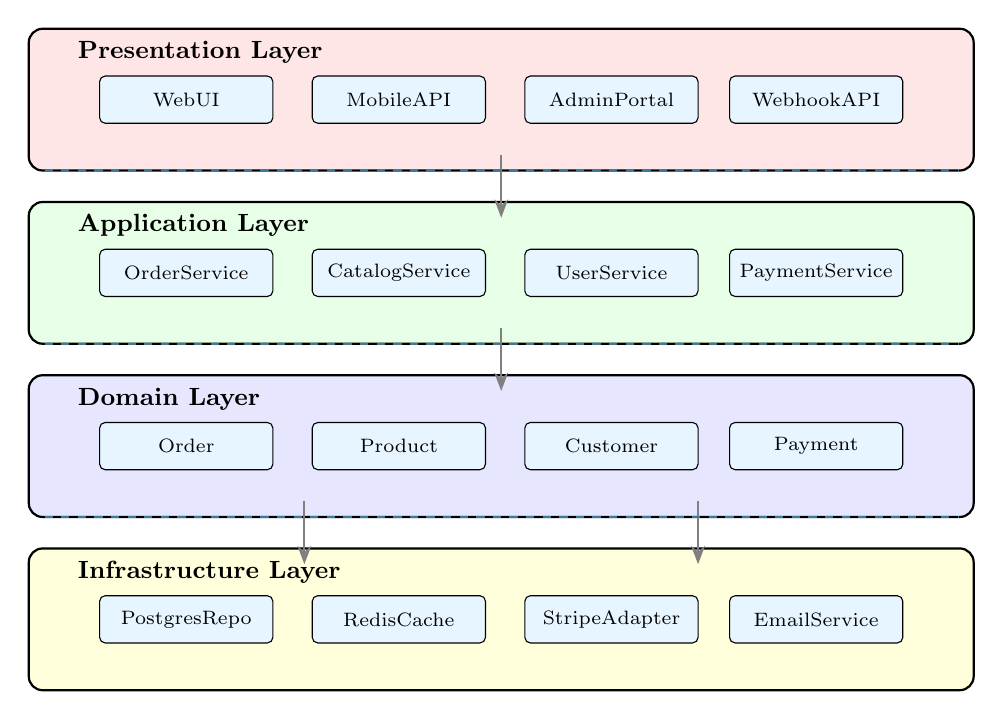
\begin{tikzpicture}[
    node distance=0.8cm,
    layer/.style={draw, thick, rounded corners=5pt, minimum width=12cm, minimum height=1.8cm},
    module/.style={draw, fill=modulecolor, rounded corners=2pt, minimum width=2.2cm, minimum height=0.6cm, font=\scriptsize},
    arrow/.style={-{Stealth}, thick, gray}
]
    % Layers
    \node[layer, fill=layercolor1] (pres) at (0, 6) {};
    \node[font=\small\bfseries, anchor=west] at (-5.5, 6.6) {Presentation Layer};
    
    \node[layer, fill=layercolor2] (app) at (0, 3.8) {};
    \node[font=\small\bfseries, anchor=west] at (-5.5, 4.4) {Application Layer};
    
    \node[layer, fill=layercolor3] (domain) at (0, 1.6) {};
    \node[font=\small\bfseries, anchor=west] at (-5.5, 2.2) {Domain Layer};
    
    \node[layer, fill=layercolor4] (infra) at (0, -0.6) {};
    \node[font=\small\bfseries, anchor=west] at (-5.5, 0) {Infrastructure Layer};
    
    % Presentation modules
    \node[module] at (-4, 6) {WebUI};
    \node[module] at (-1.3, 6) {MobileAPI};
    \node[module] at (1.4, 6) {AdminPortal};
    \node[module] at (4, 6) {WebhookAPI};
    
    % Application modules
    \node[module] at (-4, 3.8) {OrderService};
    \node[module] at (-1.3, 3.8) {CatalogService};
    \node[module] at (1.4, 3.8) {UserService};
    \node[module] at (4, 3.8) {PaymentService};
    
    % Domain modules
    \node[module] at (-4, 1.6) {Order};
    \node[module] at (-1.3, 1.6) {Product};
    \node[module] at (1.4, 1.6) {Customer};
    \node[module] at (4, 1.6) {Payment};
    
    % Infrastructure modules
    \node[module] at (-4, -0.6) {PostgresRepo};
    \node[module] at (-1.3, -0.6) {RedisCache};
    \node[module] at (1.4, -0.6) {StripeAdapter};
    \node[module] at (4, -0.6) {EmailService};
    
    % Dependency arrows
    \draw[arrow] (0, 5.3) -- (0, 4.5);
    \draw[arrow] (0, 3.1) -- (0, 2.3);
    \draw[arrow] (-2.5, 0.9) -- (-2.5, 0.1);
    \draw[arrow] (2.5, 0.9) -- (2.5, 0.1);
    
    % Interface markers
    \draw[thick, dashed, secondary] (-5.8, 5.1) -- (5.8, 5.1);
    \draw[thick, dashed, secondary] (-5.8, 2.9) -- (5.8, 2.9);
    \draw[thick, dashed, secondary] (-5.8, 0.7) -- (5.8, 0.7);
    
\end{tikzpicture}
\caption{Layered E-Commerce Application Module Structure}
\end{figure}

\textbf{Description:} This example shows a four-layer architecture for an e-commerce system. The Presentation Layer handles all external interfaces (web, mobile, admin, webhooks). The Application Layer contains use-case orchestration services. The Domain Layer holds pure business logic with no infrastructure dependencies. The Infrastructure Layer provides concrete implementations for persistence, caching, and external integrations.

\subsection{Example 2: Hexagonal Architecture}

\begin{figure}[H]
\centering
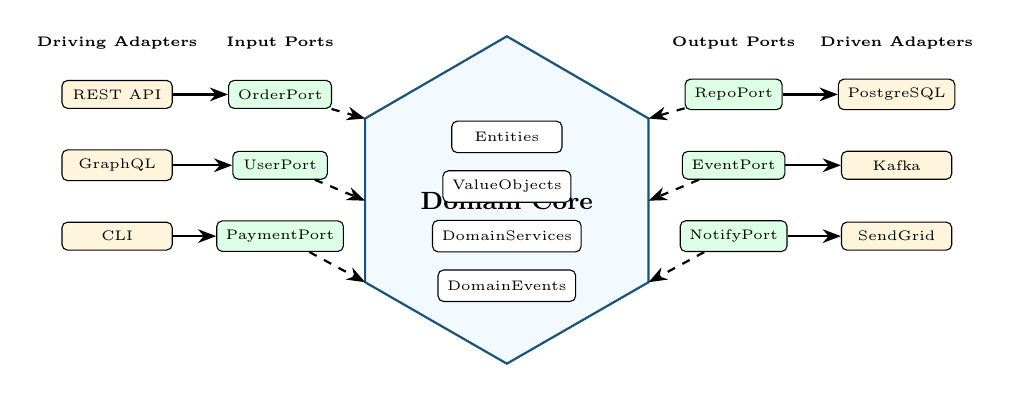
\begin{tikzpicture}[scale=0.9]
    % Core hexagon
    \fill[modulecolor!50] (0,0) -- (2,1.15) -- (2,3.46) -- (0,4.62) -- (-2,3.46) -- (-2,1.15) -- cycle;
    \draw[thick, primary] (0,0) -- (2,1.15) -- (2,3.46) -- (0,4.62) -- (-2,3.46) -- (-2,1.15) -- cycle;
    \node[font=\small\bfseries] at (0, 2.3) {Domain Core};
    
    % Core modules
    \node[draw, fill=white, rounded corners=2pt, minimum width=1.4cm, minimum height=0.4cm, font=\tiny] at (0, 3.2) {Entities};
    \node[draw, fill=white, rounded corners=2pt, minimum width=1.4cm, minimum height=0.4cm, font=\tiny] at (0, 2.5) {ValueObjects};
    \node[draw, fill=white, rounded corners=2pt, minimum width=1.4cm, minimum height=0.4cm, font=\tiny] at (0, 1.8) {DomainServices};
    \node[draw, fill=white, rounded corners=2pt, minimum width=1.4cm, minimum height=0.4cm, font=\tiny] at (0, 1.1) {DomainEvents};
    
    % Ports (interfaces)
    \node[draw, fill=interfacecolor, rounded corners=2pt, minimum width=1.2cm, minimum height=0.35cm, font=\tiny] (port1) at (-3.2, 3.8) {OrderPort};
    \node[draw, fill=interfacecolor, rounded corners=2pt, minimum width=1.2cm, minimum height=0.35cm, font=\tiny] (port2) at (-3.2, 2.8) {UserPort};
    \node[draw, fill=interfacecolor, rounded corners=2pt, minimum width=1.2cm, minimum height=0.35cm, font=\tiny] (port3) at (-3.2, 1.8) {PaymentPort};
    \node[draw, fill=interfacecolor, rounded corners=2pt, minimum width=1.2cm, minimum height=0.35cm, font=\tiny] (port4) at (3.2, 3.8) {RepoPort};
    \node[draw, fill=interfacecolor, rounded corners=2pt, minimum width=1.2cm, minimum height=0.35cm, font=\tiny] (port5) at (3.2, 2.8) {EventPort};
    \node[draw, fill=interfacecolor, rounded corners=2pt, minimum width=1.2cm, minimum height=0.35cm, font=\tiny] (port6) at (3.2, 1.8) {NotifyPort};
    
    % Driving Adapters (left)
    \node[draw, fill=packagecolor, rounded corners=2pt, minimum width=1.4cm, minimum height=0.35cm, font=\tiny] (adapt1) at (-5.5, 3.8) {REST API};
    \node[draw, fill=packagecolor, rounded corners=2pt, minimum width=1.4cm, minimum height=0.35cm, font=\tiny] (adapt2) at (-5.5, 2.8) {GraphQL};
    \node[draw, fill=packagecolor, rounded corners=2pt, minimum width=1.4cm, minimum height=0.35cm, font=\tiny] (adapt3) at (-5.5, 1.8) {CLI};
    
    % Driven Adapters (right)
    \node[draw, fill=packagecolor, rounded corners=2pt, minimum width=1.4cm, minimum height=0.35cm, font=\tiny] (adapt4) at (5.5, 3.8) {PostgreSQL};
    \node[draw, fill=packagecolor, rounded corners=2pt, minimum width=1.4cm, minimum height=0.35cm, font=\tiny] (adapt5) at (5.5, 2.8) {Kafka};
    \node[draw, fill=packagecolor, rounded corners=2pt, minimum width=1.4cm, minimum height=0.35cm, font=\tiny] (adapt6) at (5.5, 1.8) {SendGrid};
    
    % Connections
    \draw[-{Stealth}, thick] (adapt1) -- (port1);
    \draw[-{Stealth}, thick] (adapt2) -- (port2);
    \draw[-{Stealth}, thick] (adapt3) -- (port3);
    \draw[-{Stealth}, thick] (port4) -- (adapt4);
    \draw[-{Stealth}, thick] (port5) -- (adapt5);
    \draw[-{Stealth}, thick] (port6) -- (adapt6);
    
    % Port to core
    \draw[-{Stealth}, thick, dashed] (port1) -- (-2, 3.46);
    \draw[-{Stealth}, thick, dashed] (port2) -- (-2, 2.3);
    \draw[-{Stealth}, thick, dashed] (port3) -- (-2, 1.15);
    \draw[-{Stealth}, thick, dashed] (port4) -- (2, 3.46);
    \draw[-{Stealth}, thick, dashed] (port5) -- (2, 2.3);
    \draw[-{Stealth}, thick, dashed] (port6) -- (2, 1.15);
    
    % Labels
    \node[font=\tiny\bfseries, anchor=south] at (-5.5, 4.3) {Driving Adapters};
    \node[font=\tiny\bfseries, anchor=south] at (-3.2, 4.3) {Input Ports};
    \node[font=\tiny\bfseries, anchor=south] at (3.2, 4.3) {Output Ports};
    \node[font=\tiny\bfseries, anchor=south] at (5.5, 4.3) {Driven Adapters};
    
\end{tikzpicture}
\caption{Hexagonal Architecture Module Structure}
\end{figure}

\textbf{Description:} This hexagonal (ports and adapters) architecture isolates the domain core from all infrastructure concerns. Input ports define how external actors can interact with the domain. Output ports define what the domain needs from infrastructure. Adapters provide concrete implementations for both driving (API, CLI) and driven (database, messaging) sides.

\subsection{Example 3: Module Dependency Graph}

\begin{figure}[H]
\centering
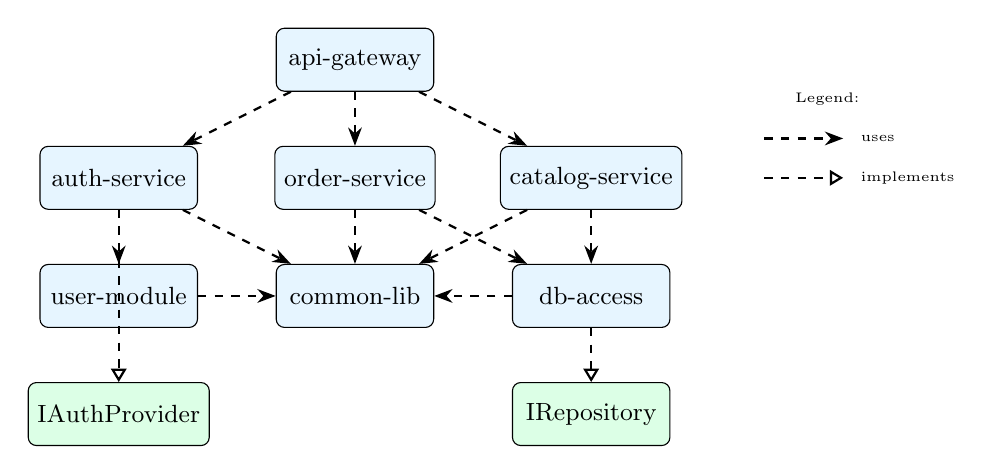
\begin{tikzpicture}[
    node distance=1.5cm and 2cm,
    module/.style={draw, fill=modulecolor, rounded corners=3pt, minimum width=2cm, minimum height=0.8cm, font=\small},
    uses/.style={-{Stealth}, thick, dashed},
    implements/.style={-{Triangle[open]}, thick, dashed}
]
    % Modules
    \node[module] (api) at (0, 4) {api-gateway};
    \node[module] (auth) at (-3, 2.5) {auth-service};
    \node[module] (order) at (0, 2.5) {order-service};
    \node[module] (catalog) at (3, 2.5) {catalog-service};
    \node[module] (user) at (-3, 1) {user-module};
    \node[module] (common) at (0, 1) {common-lib};
    \node[module] (db) at (3, 1) {db-access};
    \node[module, fill=interfacecolor] (iauth) at (-3, -0.5) {IAuthProvider};
    \node[module, fill=interfacecolor] (irepo) at (3, -0.5) {IRepository};
    
    % Dependencies
    \draw[uses] (api) -- (auth);
    \draw[uses] (api) -- (order);
    \draw[uses] (api) -- (catalog);
    \draw[uses] (auth) -- (user);
    \draw[uses] (auth) -- (common);
    \draw[uses] (order) -- (common);
    \draw[uses] (order) -- (db);
    \draw[uses] (catalog) -- (common);
    \draw[uses] (catalog) -- (db);
    \draw[uses] (user) -- (common);
    \draw[uses] (db) -- (common);
    
    % Implementations
    \draw[implements] (auth) -- (iauth);
    \draw[implements] (db) -- (irepo);
    
    % Legend
    \node[font=\tiny] at (6, 3.5) {Legend:};
    \draw[uses] (5.2, 3) -- (6.2, 3);
    \node[font=\tiny, right] at (6.3, 3) {uses};
    \draw[implements] (5.2, 2.5) -- (6.2, 2.5);
    \node[font=\tiny, right] at (6.3, 2.5) {implements};
\end{tikzpicture}
\caption{Module Dependency Graph}
\end{figure}

\textbf{Description:} This dependency graph shows the uses relationships between modules in a microservice-style application. The api-gateway depends on multiple services. Services share common utilities through common-lib. Database access is centralized in db-access. Interface modules (IAuthProvider, IRepository) define contracts that concrete modules implement.

% =============================================================================
% SECTION: NOTES
% =============================================================================
\section{Notes}

\subsection{Versioning Considerations}

Development views should evolve with the codebase:

\begin{itemize}
    \item Maintain architecture documentation in the same repository as code
    \item Update diagrams when significant structural changes occur
    \item Tag documentation versions with release versions
    \item Use architecture-as-code tools for automatic synchronization
    \item Review architecture documentation in pull requests for structural changes
\end{itemize}

\subsection{Tooling Recommendations}

\begin{table}[H]
\centering
\caption{Recommended Tools by Use Case}
\small
\begin{tabular}{@{}L{3.5cm}L{10cm}@{}}
\toprule
\textbf{Use Case} & \textbf{Recommended Tools} \\
\midrule
Diagram Creation & PlantUML, Structurizr, draw.io, Lucidchart, Mermaid \\
Architecture Validation & ArchUnit, Structure101, Sonargraph, NDepend \\
Dependency Analysis & Lattix, Understand, JDepend, madge (JS) \\
Documentation & Markdown/AsciiDoc, Confluence, GitBook \\
Code Metrics & SonarQube, CodeClimate, Codacy \\
\bottomrule
\end{tabular}
\end{table}

\subsection{Common Pitfalls}

\begin{warningbox}[Common Mistakes to Avoid]
\begin{enumerate}[nosep]
    \item \textbf{Big Ball of Mud:} Allowing unconstrained dependencies leading to unmaintainable code
    \item \textbf{Leaky Abstractions:} Exposing implementation details through interfaces
    \item \textbf{Circular Dependencies:} Creating cycles that prevent independent building/testing
    \item \textbf{God Modules:} Creating modules with too many responsibilities
    \item \textbf{Outdated Documentation:} Letting diagrams diverge from actual code
    \item \textbf{Over-Engineering:} Creating excessive abstraction layers without benefit
    \item \textbf{Ignoring Layer Violations:} Allowing shortcuts that erode architectural integrity
\end{enumerate}
\end{warningbox}

\subsection{Evolution and Refactoring}

Module structure should be continuously improved:

\begin{itemize}
    \item Monitor architectural metrics in CI/CD pipelines
    \item Establish architecture fitness functions
    \item Schedule regular architecture review sessions
    \item Maintain a technical debt backlog with structural items
    \item Use strangler fig pattern for incremental restructuring
    \item Document and communicate architectural decisions via ADRs
\end{itemize}

% =============================================================================
% SECTION: SOURCES
% =============================================================================
\section{Sources}

\subsection{Primary References}

\begin{enumerate}
    \item Clements, P., Bachmann, F., Bass, L., Garlan, D., Ivers, J., Little, R., Merson, P., Nord, R., \& Stafford, J. (2010). \textit{Documenting Software Architectures: Views and Beyond} (2nd ed.). Addison-Wesley Professional.
    
    \item ISO/IEC/IEEE 42010:2011. \textit{Systems and software engineering --- Architecture description}. International Organization for Standardization.
    
    \item Martin, R. C. (2017). \textit{Clean Architecture: A Craftsman's Guide to Software Structure and Design}. Prentice Hall.
    
    \item Vernon, V. (2013). \textit{Implementing Domain-Driven Design}. Addison-Wesley Professional.
    
    \item Object Management Group. (2017). \textit{Unified Modeling Language Specification Version 2.5.1}. OMG Document formal/2017-12-05.
\end{enumerate}

\subsection{Supplementary References}

\begin{enumerate}[resume]
    \item Parnas, D. L. (1972). On the Criteria To Be Used in Decomposing Systems into Modules. \textit{Communications of the ACM}, 15(12), 1053-1058.
    
    \item Cockburn, A. (2005). \textit{Hexagonal Architecture}. alistair.cockburn.us.
    
    \item Brown, S. (2018). \textit{The C4 Model for Visualising Software Architecture}. Leanpub.
    
    \item Ford, N., Parsons, R., \& Kua, P. (2017). \textit{Building Evolutionary Architectures}. O'Reilly Media.
    
    \item Richards, M. \& Ford, N. (2020). \textit{Fundamentals of Software Architecture}. O'Reilly Media.
\end{enumerate}

\subsection{Online Resources}

\begin{itemize}
    \item C4 Model: \url{https://c4model.com/}
    \item ArchUnit: \url{https://www.archunit.org/}
    \item PlantUML: \url{https://plantuml.com/}
    \item Structurizr: \url{https://structurizr.com/}
    \item Architecture Decision Records: \url{https://adr.github.io/}
\end{itemize}

% =============================================================================
% APPENDIX
% =============================================================================
\appendix

\section{Development View Checklist}

Use this checklist to verify completeness of development documentation:

\begin{table}[H]
\centering
\small
\begin{tabular}{@{}L{10cm}C{2cm}@{}}
\toprule
\textbf{Item} & \textbf{Complete?} \\
\midrule
\multicolumn{2}{l}{\textbf{Module Structure}} \\
\quad All major modules identified and named & $\square$ \\
\quad Module responsibilities documented & $\square$ \\
\quad Hierarchical decomposition complete & $\square$ \\
\quad Module ownership assigned & $\square$ \\
\midrule
\multicolumn{2}{l}{\textbf{Dependencies}} \\
\quad All uses relationships documented & $\square$ \\
\quad Circular dependencies identified/resolved & $\square$ \\
\quad External dependencies cataloged & $\square$ \\
\quad Dependency rationale documented & $\square$ \\
\midrule
\multicolumn{2}{l}{\textbf{Layering}} \\
\quad Layers defined with responsibilities & $\square$ \\
\quad Modules assigned to layers & $\square$ \\
\quad Layer dependency rules specified & $\square$ \\
\quad Violations identified and addressed & $\square$ \\
\midrule
\multicolumn{2}{l}{\textbf{Interfaces}} \\
\quad Public interfaces documented & $\square$ \\
\quad Interface contracts specified & $\square$ \\
\quad Versioning policy defined & $\square$ \\
\quad API documentation available & $\square$ \\
\midrule
\multicolumn{2}{l}{\textbf{Build and Organization}} \\
\quad Build structure documented & $\square$ \\
\quad Source code organization defined & $\square$ \\
\quad Build dependencies match code dependencies & $\square$ \\
\quad Artifact structure specified & $\square$ \\
\midrule
\multicolumn{2}{l}{\textbf{Validation}} \\
\quad Correspondence with C\&C view verified & $\square$ \\
\quad Architecture tests implemented & $\square$ \\
\quad Quality metrics established & $\square$ \\
\quad Review with development teams completed & $\square$ \\
\bottomrule
\end{tabular}
\end{table}

\section{Glossary}

\begin{description}[style=nextline, leftmargin=3cm, labelwidth=2.8cm]
    \item[Abstraction] The process of hiding implementation details behind a well-defined interface.
    
    \item[Cohesion] A measure of how strongly related the responsibilities within a module are.
    
    \item[Coupling] The degree of interdependence between modules.
    
    \item[Decomposition] The process of breaking a system into smaller, manageable modules.
    
    \item[Dependency] A relationship where one module requires another to function correctly.
    
    \item[Encapsulation] The bundling of data and methods that operate on that data within a single module.
    
    \item[Information Hiding] A design principle that each module should hide design decisions from other modules.
    
    \item[Interface] A contract that specifies the operations a module provides without exposing implementation.
    
    \item[Layer] A horizontal grouping of modules at the same level of abstraction.
    
    \item[Module] A code unit that bundles related functionality with a well-defined interface.
    
    \item[Package] A namespace container that organizes related modules.
    
    \item[Separation of Concerns] The principle that each module should address a distinct concern.
    
    \item[Single Responsibility Principle] A module should have only one reason to change.
    
    \item[Technical Debt] The implied cost of additional rework caused by choosing quick solutions over better approaches.
    
    \item[Uses Relationship] A dependency where one module requires the correct functioning of another.
\end{description}

\section{Module Specification Template}

\begin{lstlisting}[caption={Complete Module Specification Template}, language={}]
================================================================================
MODULE SPECIFICATION
================================================================================

1. IDENTIFICATION
-----------------
Module ID:          [MOD-XXX]
Name:               [Module Name]
Version:            [X.Y.Z]
Status:             [Draft | Review | Approved | Deprecated]
Owner:              [Team/Individual]
Last Updated:       [Date]

2. OVERVIEW
-----------
Purpose:
  [Brief description of the module's purpose]

Responsibility:
  [Primary responsibility - single sentence]

Quality Attributes:
  - Modifiability:  [High | Medium | Low]
  - Testability:    [High | Medium | Low]
  - Reusability:    [High | Medium | Low]

3. INTERFACES
-------------
Provided Interfaces:
  +------------------+------------------------------------------+
  | Interface        | Description                              |
  +------------------+------------------------------------------+
  | [InterfaceName]  | [Description of provided interface]      |
  +------------------+------------------------------------------+

Required Interfaces:
  +------------------+------------------+------------------------+
  | Interface        | Provider         | Purpose                |
  +------------------+------------------+------------------------+
  | [InterfaceName]  | [Module Name]    | [Why needed]           |
  +------------------+------------------+------------------------+

4. STRUCTURE
------------
Submodules:
  - [SubmoduleName]: [Description]
  - ...

Key Classes/Components:
  - [ClassName]: [Responsibility]
  - ...

5. DEPENDENCIES
---------------
Uses (compile-time):
  - [ModuleName]: [Reason]
  - ...

Runtime Dependencies:
  - [ModuleName]: [Reason]
  - ...

Test Dependencies:
  - [ModuleName]: [Purpose]
  - ...

External Dependencies:
  - [LibraryName] v[X.Y]: [Purpose]
  - ...

6. CONSTRAINTS
--------------
Layer Assignment:    [Layer Name]
Allowed Dependencies: [List of allowed modules/layers]
Prohibited:          [Any specific prohibitions]

7. RATIONALE
------------
Design Decisions:
  - [Decision 1]: [Rationale]
  - [Decision 2]: [Rationale]

Alternatives Considered:
  - [Alternative]: [Why rejected]

8. METRICS
----------
Lines of Code:       [Approximate]
Cyclomatic Complexity: [Average]
Test Coverage:       [Percentage]
Dependencies In:     [Count]
Dependencies Out:    [Count]

9. CHANGE HISTORY
-----------------
[Date] - [Version] - [Author] - [Description of change]

================================================================================
\end{lstlisting}

% =============================================================================
% END DOCUMENT
% =============================================================================

\end{document}
